\documentclass[11pt]{article}
\usepackage[margin=1.1in]{geometry}
\usepackage{amsmath,amssymb,amsthm}
\usepackage{mathpazo}
\usepackage{microtype}
\usepackage{tikz}
\usetikzlibrary{calc,arrows.meta}
\usepackage[hidelinks]{hyperref}

\newtheorem{proposition}{Proposition}
\theoremstyle{definition}
\newtheorem{definition}{Definition}
\theoremstyle{remark}
\newtheorem*{remark}{Remark}

\newcommand{\R}{\mathbb{R}}
\newcommand{\E}{\mathbb{E}}
\newcommand{\A}{\mathcal{A}}

\title{The Shape of Search\\[4pt]
\large Reachability, Measurement, and Attraction in Physical, Cognitive, and Conversational Systems}
\author{Flyxion\\ Independent Researcher}
\date{September 2026}

\begin{document}
\maketitle

\begin{abstract}
Systems are routinely characterized by where they end up: an optimizer by the minimum it reports, a participant by a fitted capacity parameter, a pair of dialogue agents by the consensus they reach. This essay argues that such endpoint descriptions omit three structures that are not annotations on the state but conditions of its intelligibility: the transition dynamics that make configurations reachable, the measurement operator through which a state becomes observable, and the attractor structure that shapes trajectories independently of the interactions supposed to drive them. Three recent empirical results supply one missing term each. A 96,000-spin CMOS-integrated voltage-controlled MRAM Ising machine realizes probabilistic spin updates directly in the pulse-width-dependent switching statistics of magnetic tunnel junctions, making the transition kernel a material property. A cross-paradigm estimation of visual processing capacity under the Theory of Visual Attention shows that a nominally task-independent parameter does not transport cleanly across tasks. A Bayesian decomposition of opinion dynamics among large language models shows rapid convergence to shared attractors that are largely explained by prior bias rather than interaction. None of these systems is claimed to instantiate a common mechanism. They expose a common inferential insufficiency, summarized by the composition $y_t = M(K^t(x_0))$: what is observed is a measurement of an iterated transition, and neither the state, nor the reading, nor the destination determines the other two.
The resulting account is positioned against bisimulation, lumpability, measurement invariance, energy-landscape theory, and classical opinion dynamics. Its claim is that state descriptions are lossy quotients of dynamical systems, and that different quotients preserve different claims.
\end{abstract}

\section{The Endpoint Fallacy}

Scientific description has a strong bias toward endpoints. A combinatorial optimizer is evaluated by the quality of the configuration it returns. A cognitive test yields a number that is filed as a property of the person tested. A simulated conversation between language models is summarized by whether the agents agreed. In each case the endpoint invites an ontological reading: the minimum is the solution, the parameter is the capacity, the consensus is the product of persuasion.

The inference is natural because endpoints are what instruments deliver. It is also systematically incomplete. A reported minimum says nothing about which other minima were reachable and under what schedule. A fitted parameter says nothing about how much of its value belongs to the task that elicited it. A shared final opinion says nothing about whether the agents moved each other or merely moved, together, down a slope that was already present before they spoke.

The general form of the problem is compact:
\begin{equation}
\text{observed trajectory} \;\neq\; \text{underlying dynamics}.
\end{equation}
The remainder of the essay develops this inequality through three cases drawn from unrelated fields. The cases are not offered as metaphors for one another. Each supplies empirical evidence for a distinct term that endpoint descriptions leave out.

Because the argument moves between reported findings and claims built on them, the status of each claim is kept visible. Results reported by the three studies are attributed to their authors. Statements that follow from definitions are stated as propositions or marked as consequences, with proofs collected in the appendix. Readings that go beyond what a source reports are marked as interpretations or inferences. New constructions, such as the continuation structure and recoverability, are introduced as definitions or proposals. Where a sentence could be taken as a finding of a cited study but is not, the text says so.

\section{Search Is Not Enumeration}

The textbook statement of optimization begins with a configuration space $X$ and an objective, or Hamiltonian, $E : X \to \R$, and asks for
\begin{equation}
x^\star \in \arg\min_{x \in X} E(x).
\end{equation}
This notation specifies where the answer lies and suppresses everything about how configurations become reachable. For any problem large enough to be interesting, enumeration is unavailable, and what actually runs is a stochastic process. Let
\begin{equation}
K_T(x' \mid x)
\end{equation}
denote a transition kernel parametrized by a control variable $T$, conventionally called temperature. An optimizer is then better described by the triple
\begin{equation}
(X, E, K_T),
\end{equation}
and two machines implementing the identical objective can execute radically different searches. The first distinction the essay requires is therefore
\begin{equation}
\text{solution space} \;\neq\; \text{search geometry}.
\end{equation}
The distinction can be stated in two forms that will recur. Two machines can share an objective and differ in kernel,
\begin{equation}
E_1 = E_2 \;\not\Rightarrow\; K_1 = K_2 ,
\end{equation}
and within one machine, two configurations can share an energy and differ in what they can become,
\begin{equation}
E(x) = E(y) \;\not\Rightarrow\; \Gamma(x) \cong \Gamma(y).
\end{equation}
Energy geometry and continuation geometry are related but not identical objects (Figure~\ref{fig:height}). The first is a scalar field on $X$. The second is a relation on $X$, fixed only once an update rule, a schedule, and a physical source of chance have been chosen. The landscape defined by $E$ does not move. What moves is a probability measure over $X$, and the kernel decides how.

\begin{figure}[t]
\centering
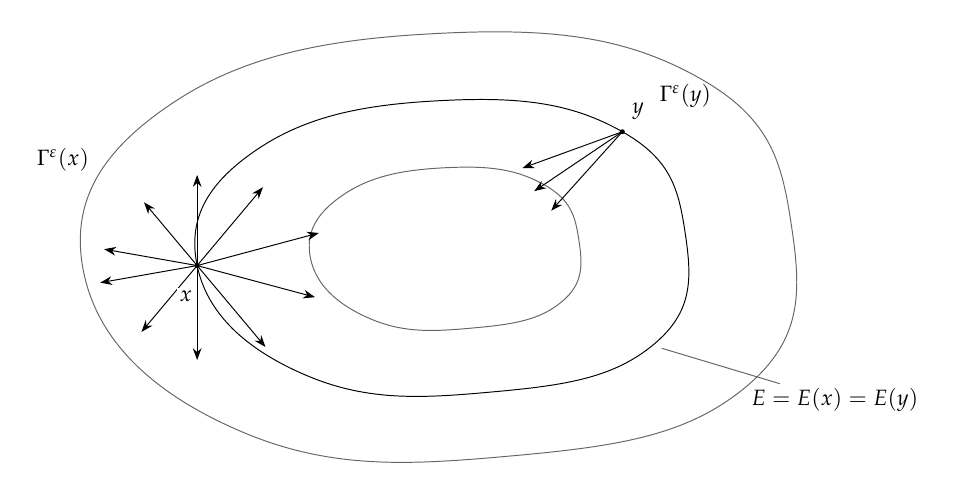
\begin{tikzpicture}[line width=0.35pt, >={Stealth[length=1.5mm,width=1.1mm]}, font=\footnotesize]
\foreach \s/\g in {0.55/60,1/100,1.45/60}{
  \draw[black!\g] plot[smooth cycle, tension=0.75] coordinates {({\s*3},{\s*0.2}) ({\s*2.2},{\s*1.5}) ({\s*0},{\s*1.9}) ({\s*-2.4},{\s*1.3}) ({\s*-3.2},{\s*-0.2}) ({\s*-1.8},{\s*-1.6}) ({\s*0.6},{\s*-1.8}) ({\s*2.6},{\s*-1.2})};
}
\coordinate (x) at (-3.2,-0.2);
\coordinate (y) at (2.2,1.5);
\foreach \a/\l in {-170/1.25,-130/1.1,-90/1.2,-50/1.35,-15/1.55,15/1.6,50/1.3,90/1.15,130/1.05,170/1.2}{
  \draw[->] (x) -- ++(\a:\l);
}
\foreach \a in {200,214,228}{
  \draw[->] (y) -- ++(\a:1.35);
}
\fill (x) circle (0.9pt); \fill (y) circle (0.9pt);
\node[inner sep=1pt, fill=white] at ($(x)+(-110:0.42)$) {$x$};
\node[anchor=south west, inner sep=2pt] at ($(y)+(0.05,0.08)$) {$y$};
\node at (4.9,-1.9) {$E = E(x) = E(y)$};
\draw[black!60] (4.2,-1.7) -- (2.7,-1.25);
\node[anchor=east] at (-4.45,1.15) {$\Gamma^{\varepsilon}(x)$};
\node[anchor=west] at (2.55,1.95) {$\Gamma^{\varepsilon}(y)$};
\end{tikzpicture}
\caption{Same height, different continuation geometry. The closed curves are level sets of $E$; $x$ and $y$ lie on the same one. Arrows mark the moves each configuration can make with probability at least $\varepsilon$. The energy function assigns the two points the same value and says nothing about the difference between their continuation sets: $E(x)=E(y) \not\Rightarrow \Gamma^{\varepsilon}(x) \cong \Gamma^{\varepsilon}(y)$. Schematic.}
\label{fig:height}
\end{figure}

\section{A Minimum Is a Relation}

A local minimum is ordinarily described as a feature of the landscape. Operationally it is a feature of the landscape relative to a transition rule. A configuration surrounded by higher energy is a trap only for a process that cannot, or will rarely, accept energetically unfavorable moves.

The voltage-controlled spintronic Ising machine (VSIM) reported by Li, Zhang, and colleagues makes this relation concrete \cite{li2026}. Its spins $s_i \in \{-1, +1\}$ are coupled through a fully connected Hamiltonian
\begin{equation}
H = -\sum_{i<j} J_{ij} s_i s_j - \sum_i h_i s_i ,
\end{equation}
and are updated under the Glauber rule \cite{glauber1963}, in the form the authors take from Mackenzie and Young \cite{mackenzie1983}. Writing $\delta H_i$ for the reduction in $H$ that flipping spin $i$ would produce,
\begin{equation}
\delta H_i = -2 s_i \Big( \sum_j J_{ij} s_j + h_i \Big), \qquad
P_{\mathrm{flip}}(\delta H_i, T) = \frac{1}{1 + e^{-\delta H_i / T}} .
\end{equation}
A flip that raises the energy has $\delta H_i < 0$ and is still accepted with appreciable probability when $T$ is large, so the process can leave basins that a greedy descent would never exit. In the routing demonstration, $T$ falls exponentially over a thousand iterations, and the measured flip rate, the fraction of spins flipping per iteration, falls from roughly one half, the high-temperature limit of the rule, toward zero.

It is useful to name the set of places a configuration can go. Because a Glauber kernel assigns positive probability to every single-spin flip at any positive temperature, bare support is uninformative. The relevant object is a thresholded continuation set:
\begin{definition}[$\varepsilon$-continuation set]
For $x \in X$, temperature $T$, and threshold $\varepsilon > 0$,
\begin{equation}
\Gamma_T^{\varepsilon}(x) = \{ x' \in X : K_T(x' \mid x) \geq \varepsilon \}.
\end{equation}
\end{definition}
A configuration is a practical minimum at $(T,\varepsilon)$ when every element of $\Gamma_T^{\varepsilon}(x)$ other than $x$ lies at higher energy and none leads, within a relevant horizon, to lower energy elsewhere. Minimality is then a joint property of $H$, $K_T$, the schedule, and the resolution $\varepsilon$ at which rare moves are treated as unavailable. Hence the governing inequality of this section:
\begin{equation}
x_t \;\not\Rightarrow\; \Gamma_t(x_t) \qquad \text{without specification of } K_t .
\end{equation}
Knowing where the system is does not determine where it can go. In a fully specified system, $x_t$ together with the kernel in force at time $t$ does fix the continuation set; the point is that the coordinate alone, detached from kernel, schedule, and implementation, does not.

\section{Probability as a Material Property}

In conventional stochastic hardware, a probability is assembled. A device or generator produces fair bits; enough of them are concatenated into a random number; the number is compared against a threshold computed through a sigmoid lookup table. The authors note that producing a single 16-bit random number from a 50/50 magnetic device takes 16 successive cycles, together with peripheral circuitry for the comparison \cite{li2026}. Chance is a raw material from which each probability must be built.

The VSIM removes the assembly. Each spin is a perpendicular magnetic tunnel junction driven by the voltage-controlled magnetic anisotropy (VCMA) effect. A voltage pulse across the MgO barrier lowers the energy barrier between the parallel and antiparallel states, the free layer precesses on a sub-nanosecond scale, and whether it ends in the opposite state depends on the pulse width $W_v$. A thick barrier suppresses spin-transfer torque, so switching is driven by electric field rather than current, and an integrated orthogonal bias layer makes the switching nearly symmetric: the same pulse flips a parallel junction and an antiparallel one with essentially the same probability, so no reset is needed before an update. Measured over a thousand repetitions per setting, the switching probability follows a sigmoid in pulse width,
\begin{equation}
P_{\mathrm{sw}}(W_v) = \frac{1}{1 + e^{-\alpha (W_v - W_0)}},
\end{equation}
with pulses of $0.5$, $0.65$, and $0.8$\,ns at $2.2$\,V giving roughly $2\%$, $55\%$, and $95\%$. Setting $P_{\mathrm{sw}} = P_{\mathrm{flip}}$ and solving yields the pulse width that realizes a Glauber update:
\begin{equation}
W_v = \frac{\delta H}{\alpha T} + W_0 .
\end{equation}

This equation is the conceptual center of the machine. Three different kinds of thing are written into one scalar: the problem, through $\delta H$; the schedule, through $T$; and the matter, through the fitted device constants $\alpha$ and $W_0$. The chain of dependence runs
\begin{equation}
(\delta H, T) \;\longmapsto\; W_v \;\longmapsto\; P_{\mathrm{sw}} = P_{\mathrm{flip}} \;\longmapsto\; K_T \;\longmapsto\; \Gamma_T^{\varepsilon}.
\end{equation}
A pulse is not storing a bit. It is setting a probability measure over the next configuration of the system.

The division of labor deserves precision, because it qualifies any claim that matter has absorbed the algorithm. In the demonstrated system, an FPGA computes $\delta H$ by matrix-vector multiplication, applies the schedule, and configures the on-chip pulse generator; the junction holds the spin and performs the Bernoulli trial. Valuation is digital; chance is magnetic. The single-spin update completes in $0.3$ to $1$\,ns at under $40$\,fJ, but the end-to-end iteration takes about $45$\,ns because of the FPGA fabric. The chip itself is a $96$-kb VC-MRAM in a $40$-nm CMOS process with junctions about $70$\,nm across, and on a standardized 60-node dense Max-cut benchmark the system reaches $1.92 \times 10^5$ solutions per second per watt, which the authors report as $60$ to $18{,}000$ times better than the competing platforms they compare. The coincidence achieved is partial but real: the element that represents the state is the element that supplies the transition, and the control parameter reaches it directly as a physical duration.

Two further results bear on the geometry of the kernel. First, probability resolution matters. Benchmarked against linear-feedback shift registers on the routing problem, the junctions reach success probabilities comparable to a 16-bit register, while 8-bit and 4-bit registers do worse. On a natural reading of this result, which the authors present as a hardware comparison, a kernel that can express only a few probability levels searches a coarser geometry than one that can express many. Second, the search tolerates heterogeneity. About a fifth of measured devices reach a peak switching probability below $90\%$; in an FPGA emulation of this variation, success probability stays above $95\%$ even when a fifth of the spins top out at $60\%$. The result suggests that what the search requires is not exact probabilities but enough of them, placed well enough, often enough.

\section{Constraint Becomes Geometry}

Real optimization problems are rarely unconstrained. Global routing in the paper is formulated as a rectilinear Steiner minimum tree (RSMT) problem: connect a set of terminal pins, possibly through auxiliary Steiner vertices, with a tree of minimum total edge cost. The Hamiltonian is a weighted sum of an objective and four penalties,
\begin{equation}
H_{\mathrm{RSMT}} = H_o + \lambda_1 H_{c1} + \lambda_2 H_{c2} + \lambda_3 H_{c3} + \lambda_4 H_{c4}.
\end{equation}
The objective $H_o$ is total edge cost. The first penalty requires every non-root terminal to have exactly one incoming arc,
\begin{equation}
H_{c1} = \sum_{v \in U \setminus \{v_0\}} \Big( 1 - \sum_{(u,v) \in E} x^e_{u,v} \Big)^2 ,
\end{equation}
and the other three, as given in the paper's supplementary material \cite{li2026}, are
\begin{align}
H_{c2} &= \sum_{\substack{u<v<w\\ u,v,w \neq v_0}} \big( x^o_{u,w} + x^o_{u,v} x^o_{v,w} - x^o_{u,v} x^o_{u,w} - x^o_{u,w} x^o_{v,w} \big)
+ \sum_{\substack{u<v\\ u,v \neq v_0}} \big( x^e_{u,v}(1 - x^o_{u,v}) + x^e_{v,u}\, x^o_{u,v} \big), \\
H_{c3} &= |V| \sum_{v \in W} \sum_{\{u,w\}} x^e_{u,v} x^e_{w,v} + \sum_{v \in W} \Big( 1 - \sum_{u} x^e_{u,v} \Big) \Big( \sum_{u} x^e_{v,u} \Big), \\
H_{c4} &= \sum_{(u,v) \in E,\ v \neq v_0} r_{u,v}\, x^e_{u,v},
\end{align}
where $W$ is the set of Steiner vertices and $r_{u,v} = 1$ when $u$ and $v$ cannot be joined by a straight rectilinear segment. The acyclicity term has two parts: the first penalizes intransitive orderings, and the second penalizes any edge that points against the ordering. The third term penalizes Steiner vertices with several incoming arcs, and Steiner vertices with outgoing arcs but none incoming; the fourth penalizes non-rectilinear connections.

The encoding contains a detail that is easy to pass over. Alongside edge variables $x^e_{u,v}$, which say whether an edge is in the tree, there are order variables $x^o_{u,v}$, which say whether $u$ is closer to the root than $v$. The order variables are not part of the answer; a routed tree is fully described by its edges. They exist because this formulation enforces acyclicity through a transitive ordering, which the edge variables alone cannot express. To make a constraint expressible as energy, the configuration space had to be enlarged with coordinates whose only purpose is to make admissibility writable. Spins are then obtained by $s = 2x - 1$, and the resulting instance has $450$ spins at $4\%$ graph density.

A logical specification would separate the representable space $X$ from an admissible subset
\begin{equation}
\A = \{ x \in X : C_1(x) \wedge C_2(x) \wedge C_3(x) \wedge C_4(x) \},
\end{equation}
and would treat $X \setminus \A$ as forbidden. The Ising formulation forbids nothing. Each constraint $C_i$ is compiled into a term $H_{ci}$ that is zero on satisfying configurations and positive otherwise, and the weighted sum deforms the landscape on which the kernel acts:
\begin{equation}
C_i \;\longrightarrow\; H_{ci} \;\longrightarrow\; H \;\longrightarrow\; \delta H \;\longrightarrow\; W_v \;\longrightarrow\; \Pr(x_{t+1} \mid x_t).
\end{equation}
In this machine the chain ends in a pulse duration. A logical condition on trees becomes, after four translations, a number of picoseconds. The admissible subspace is not a region cut out of $X$ but a basin carved into it.

State-level admissibility is a special case of a finer notion. Admissibility can be graded and assigned to transitions rather than states, as a function
\begin{equation}
\mathrm{Adm} : X \times X \to [0,1],
\end{equation}
with a transition counted admissible when $\mathrm{Adm}(x, x') \geq \theta$ for a contextually fixed threshold \cite{flyxion-clipboard}. The set $\A$ corresponds to the degenerate choice $\mathrm{Adm}(x, x') = \mathbf{1}[x' \in \A]$. With transition admissibility in hand, three sets that are easily run together come apart:
\begin{equation}
\underbrace{X}_{\text{possible}} \;\supseteq\; \underbrace{\Gamma^{\varepsilon}(x)}_{\text{reachable}} \;\supseteq\; \underbrace{\Gamma^{\varepsilon,\theta}(x) = \{x' \in \Gamma^{\varepsilon}(x) : \mathrm{Adm}(x,x') \geq \theta\}}_{\text{admissibly reachable}} .
\end{equation}
The set-level version of this distinction, between continuations reachable from a state and those admitted by the surrounding arrangement, and further between nominal admission as specified and effective admission as realized, was developed earlier for assembled AI systems \cite{flyxion-arranged}; the present chain adds a probability threshold to reachability and a grade to admissibility. A penalty formulation is, in these terms, a decision to keep the middle set strictly larger than the last (Figure~\ref{fig:nested}). Configurations that fail the constraints remain reachable by design, and the next section argues that the search makes use of them and, for some changes between valid trees, cannot avoid them.

\begin{figure}[t]
\centering
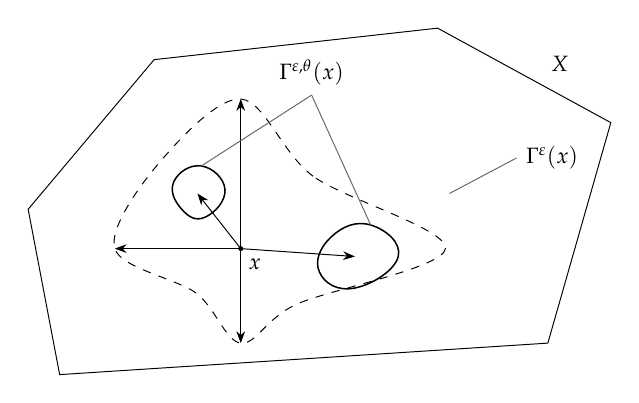
\begin{tikzpicture}[line width=0.35pt, >={Stealth[length=1.5mm,width=1.1mm]}, font=\footnotesize]
\draw (0,0) -- (6.2,0.4) -- (7,3.2) -- (4.8,4.4) -- (1.2,4.0) -- (-0.4,2.1) -- cycle;
\node at (6.35,3.95) {$X$};
\coordinate (x) at (2.3,1.6);
\draw[dashed] plot[smooth cycle, tension=0.55] coordinates {($(x)+(0:2.6)$) ($(x)+(45:1.3)$) ($(x)+(90:1.9)$) ($(x)+(135:1.5)$) ($(x)+(180:1.6)$) ($(x)+(225:0.8)$) ($(x)+(270:1.2)$) ($(x)+(315:1.0)$)};
\draw[line width=0.55pt] plot[smooth cycle, tension=0.8] coordinates {(4.3,1.5) (3.95,1.9) (3.45,1.75) (3.3,1.3) (3.75,1.1)};
\draw[line width=0.55pt] plot[smooth cycle, tension=0.8] coordinates {(2.1,2.35) (1.8,2.65) (1.45,2.45) (1.55,2.1) (1.85,2.0)};
\foreach \a/\r in {90/1.9,180/1.6,270/1.2}{
  \draw[->] (x) -- ($(x)+(\a:\r)$);
}
\draw[->] (x) -- (3.75,1.5);
\draw[->] (x) -- (1.75,2.3);
\fill (x) circle (0.9pt);
\node[anchor=north, inner sep=2pt] at ($(x)+(0.18,-0.05)$) {$x$};
\draw[black!60] (4.95,2.3) -- (5.8,2.75) node[anchor=west, black] {$\Gamma^{\varepsilon}(x)$};
\node[anchor=south] (lab) at (3.2,3.55) {$\Gamma^{\varepsilon,\theta}(x)$};
\draw[black!60] (lab.south) -- (3.95,1.9);
\draw[black!60] (lab.south) -- (1.8,2.65);
\end{tikzpicture}
\caption{Possible, reachable, admissibly reachable. The outer polygon is the representable space $X$; the dashed star is the set reachable from $x$ with probability at least $\varepsilon$; the two solid regions are the admissibly reachable subset, which need not be connected and need not contain $x$. Rays ending at the dashed boundary are reachable but not admissible. $X \supseteq \Gamma^{\varepsilon}(x) \supseteq \Gamma^{\varepsilon,\theta}(x)$. Schematic.}
\label{fig:nested}
\end{figure}

\section{Occupied Invalidity}

A consequence of this conversion is that invalid states are visited, and not rarely. The paper classifies outcomes as optimal trees, valid but suboptimal trees, and invalid solutions with unconnected terminals, and tracks their proportions across iterations over a hundred independent trials per setting. Early in annealing, invalid outcomes are the majority. Their share falls as iterations accumulate, and beyond about $10^4$ iterations the optimal tree is found in more than $95\%$ of trials at the baseline weights $\lambda_1 = \lambda_2 = 10$, $\lambda_3 = \lambda_4 = 6$. Snapshots of a single run show the route passing from a random configuration through suboptimal trees to the optimum in its final few dozen iterations. Invalidity is not an exceptional failure. It is a phase of the process.
\begin{equation}
\text{invalidity} \;\neq\; \text{absence}.
\end{equation}
An invalid configuration can be occupied, measured, classified, and left. A search forbidden ever to enter $X \setminus \A$ would have to move between valid trees using only valid intermediates. Under single-spin moves in this encoding, some elementary changes between valid trees necessarily pass through invalid intermediates: re-parenting a terminal, or a Steiner vertex with children, means exchanging its incoming arc for another, which takes at least two flips, and after the first flip that vertex has either two incoming arcs or none, violating the in-degree penalties or detaching part of the tree. Order variables that must be updated alongside the edges add further intermediate violations. The argument concerns the encoding, not a measurement reported in the paper.

The penalty-sensitivity analysis refines this picture considerably \cite{li2026}. Varying one coefficient at a time from the baseline:
low $\lambda_1$, $\lambda_2$, or $\lambda_3$ produces mostly invalid solutions;
low $\lambda_4$ produces mostly valid but suboptimal trees, and at $\lambda_4 = 0$ the optimum almost never appears;
high $\lambda_1$ shifts outcomes from optimal toward suboptimal trees;
high $\lambda_3$ increases the share of invalid solutions;
high $\lambda_2$ or $\lambda_4$ does little harm.
Three lessons follow.

First, there is no single axis called penalty strength. Each constraint has its own response profile, and the relation between weight and outcome is not
\begin{equation}
\lambda \uparrow \;\Rightarrow\; \text{better},
\end{equation}
but rather
\begin{equation}
(\lambda_1, \ldots, \lambda_4) \;\longmapsto\; \text{shape of the accessible low-energy region}.
\end{equation}

Second, a heavier penalty can produce more invalid outcomes, and this cannot be a fact about where the minimum lies. Every penalty term is nonnegative and vanishes on configurations that satisfy its constraint; for $H_{c3}$, whose second part can be negative, the weight $|V|$ on the first part restores nonnegativity (Proposition~\ref{prop:penalty}). Raising one weight leaves the energy of every admissible configuration that satisfies the corresponding constraint unchanged and raises or preserves the energy of everything else, so a global minimizer that lay in $\A$ before the change still lies there afterward (Proposition~\ref{prop:penalty}). Provided the baseline ground state is the optimal tree, which the success rate above $95\%$ at baseline weights suggests but does not prove, increasing $\lambda_3$ cannot have moved it. The authors' own explanation is that a large $\lambda_3$ reduces the relative importance of $\lambda_1$ and $\lambda_2$, making failure to form a valid tree more likely. Relative importance can only matter dynamically, since the minimizer is fixed. The most direct dynamical reading, which is an interpretation rather than a reported finding, is that the landscape between here and there has changed: new basins that satisfy the heavily weighted constraint while violating others, separated from the admissible optimum by barriers that a finite schedule does not cross. Invalid endpoints under heavy penalties are failures of reachability, not of specification.

Third, raising and lowering a penalty are not symmetric. Raising a weight cannot move an admissible ground state; lowering one can, because configurations that violate the relaxed constraint become cheaper. Setting $\lambda_4$ near zero does not produce invalid trees; it produces trees classified as suboptimal. The simplest reading is static: without the rectilinearity penalty, the ground state of the relaxed Hamiltonian may itself use connections that the routing evaluation counts against it. That reading is an inference, not a result reported in the paper, and it exposes something the outcome classes conceal. The paper's category of invalid solutions refers to unconnected terminals, while rectilinearity violations appear to fall under suboptimal trees. If so, the admissible set used to score outcomes is not simply the intersection of the four encoded constraints, and what counts as failure depends on which constraints the evaluation treats as defining validity. Two specifications of admission are in play, one encoded in the Hamiltonian and one applied when outcomes are scored, and they need not coincide.

The supplementary material states the authors' reading of the other two coefficients. A large $\lambda_1$ creates a conflict between minimizing cost and satisfying the constraint that limits exploration of better solutions; large $\lambda_2$ and $\lambda_4$ are harmless because those constraints do not conflict with the objective or with each other \cite{li2026}.

The mechanism proposed here for the tradeoff at high $\lambda_1$, barrier inflation between valid configurations, is an interpretation rather than a claim of the paper, though it is consistent with the authors' description of limited exploration. The general point does not depend on that mechanism, though it is a proposal the outcome data support rather than a result they report. A boundary does not merely separate good states from bad. Its implementation redistributes error among three kinds: ending outside the admissible set, ending inside it at the wrong place, and never arriving at all within the time allowed.

\section{Competing Valuations}

Layer assignment sharpens the point by replacing the opposition between objective and constraint with an opposition between two objectives. In a four-layer model, horizontal segments occupy layers $L_1$ or $L_3$ and vertical segments $L_2$ or $L_4$, and each segment's spin chooses between its two layers. A density term rewards placing overlapping nearby segments on different layers, with local density $w_{ij} = l/d$ for overlap length $l$ and separation $d$; it is a Max-cut problem. A via term penalizes the layer changes needed where horizontal and vertical segments connect. The combined Hamiltonian is
\begin{equation}
H_{\mathrm{DVLA}} = \lambda_D H_D + \lambda_v H_v ,
\end{equation}
and the two terms pull against each other: spreading wires across layers to reduce density tends to require more vias \cite{li2026}. With $\lambda_D = 10$ and $\lambda_v = 4$, the optimality gap falls below $2\%$ beyond about $10^4$ iterations for problems of $20$ to $100$ segments.

No configuration of the chip changes when the ratio $\lambda_D / \lambda_v$ changes. What changes is which configurations are neighbors in the sense that matters to the kernel. Writing $\widetilde{X}$ for the configuration space equipped with the effective adjacency induced by the weighted Hamiltonian,
\begin{equation}
X \xrightarrow{\;\{H_i, \lambda_i\}\;} \widetilde{X}.
\end{equation}
The physical states are fixed. Their effective proximity is not.
Search does not merely rank destinations. It manufactures adjacency: which parts of $X$ count as next to the present state is decided by weights, temperature, and device, not by $X$.

The paper records a small fact that makes the same point from another side. Because of the Max-cut form of $H_D$, the total Hamiltonian is negative when $\lambda_D$ greatly exceeds $\lambda_v$, and the authors remark that this is harmless, since only relative variation matters. The kernel sees only $\delta H / T$. Adding a constant to the landscape changes nothing, and scaling the landscape together with the temperature changes nothing:
\begin{equation}
(H, T) \;\sim\; (cH + d,\; cT), \qquad c > 0 .
\end{equation}
The height of the landscape is not an observable of the search. What the search experiences is a set of energy differences measured in units of the current temperature, and in this machine, measured in the end as pulse durations.

\section{Adverse Transitions}

At high temperature the machine deliberately accepts flips that raise the Hamiltonian, and the recorded energy trajectory shows occasional increases against a downward trend. Judged move by move, these are errors. Judged as part of a trajectory, they are how the process escapes basins that do not contain good solutions. Thus
\begin{equation}
\delta H < 0 \;\not\Rightarrow\; \text{error}.
\end{equation}
The example motivates separating three levels at which failure can be assessed:
\begin{equation}
\text{error of state} \;\neq\; \text{error of transition} \;\neq\; \text{error of process}.
\end{equation}
A configuration can be invalid while the transition that produced it was appropriate, as when an uphill move is accepted early in annealing. A transition can be locally adverse, intentionally permitted, and globally necessary. A process can reach a good state by a path that would not reliably reach it again, which is why the paper reports success probabilities over a hundred trials rather than single runs. Evaluation that attends only to states conflates the three, and in doing so misclassifies the exploratory component of any search that works.

\section{Annealing as Scheduled Loss of Alternatives}

Annealing is usually narrated as cooling. It can equally be described as a schedule for the contraction of alternatives. For an uphill move with fixed $\delta H < 0$, the Glauber probability decreases monotonically as $T$ decreases. It follows that for any threshold $\varepsilon$, the uphill portion of the continuation set is nested along a decreasing schedule:
\begin{equation}
\Gamma_{T_0}^{\varepsilon,-}(x) \supseteq \Gamma_{T_1}^{\varepsilon,-}(x) \supseteq \cdots \supseteq \Gamma_{T_n}^{\varepsilon,-}(x), \qquad T_0 > T_1 > \cdots > T_n,
\end{equation}
where the superscript restricts to moves with $\delta H < 0$. Downhill moves become more probable as $T$ falls, so the contraction is directional: the process loses the ability to go up while retaining, and strengthening, the ability to go down (Proposition~\ref{prop:nest}; Figure~\ref{fig:anneal}).

In the VSIM this contraction has a physical signature. Since $W_v - W_0 = \delta H / (\alpha T)$, lowering the temperature pushes the pulse widths required for any fixed energy change away from $W_0$, toward the short pulses that almost never switch and the long pulses that almost always do. The writable window, from $0.3$ to $1$\,ns, eventually clips them. It follows from the pulse-width equation that, late in annealing, updates with energy changes of any appreciable size are pushed toward the edges of what the pulse generator can produce, where the switching curve is nearly flat at zero or one. How large a share of late updates this covers depends on the distribution of energy changes and the schedule, which the paper does not report. To that extent, the final commitments of the search are made where the device's range of expressible probabilities runs out.

Early search preserves alternatives; late search suppresses them. Convergence then reads as
\begin{equation}
\text{exploration} \;\longrightarrow\; \text{restriction} \;\longrightarrow\; \text{commitment}.
\end{equation}
Described this way, the art of annealing is not the art of finding low places. It is the art of deciding when possibilities stop being possibilities. A schedule that contracts too early commits to the first basin; one that contracts too late never commits. The quality of the answer is a property of the timing of loss.

\begin{figure}[t]
\centering
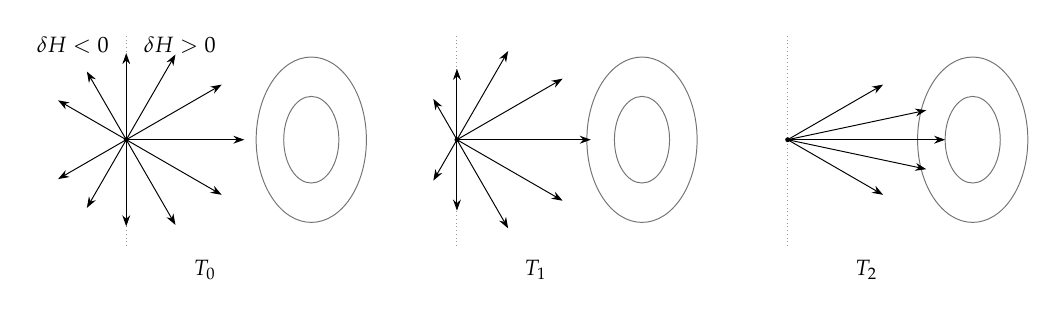
\begin{tikzpicture}[line width=0.35pt, >={Stealth[length=1.4mm,width=1mm]}, font=\footnotesize]
\newcommand{\panel}[3]{% #1 xshift, #2 uphill angle list, #3 label
  \begin{scope}[xshift=#1 cm]
    \coordinate (a) at (0,0);
    \draw[black!55] (2.35,0) ellipse (0.35 and 0.55);
    \draw[black!55] (2.35,0) ellipse (0.7 and 1.05);
    \draw[black!40, densely dotted] (0,-1.35) -- (0,1.35);
    #2
    \fill (a) circle (0.9pt);
    \node at (1,-1.65) {#3};
  \end{scope}}
\panel{0}{\foreach \t/\l in {-150/1.0,-120/1.0,150/1.0,120/1.0,-90/1.1,90/1.1,-60/1.25,60/1.25,-30/1.4,30/1.4,0/1.5}{\draw[->] (a) -- ++(\t:\l);}}{$T_0$}
\panel{4.2}{\foreach \t/\l in {-120/0.6,120/0.6,-90/0.9,90/0.9,-60/1.3,60/1.3,-30/1.55,30/1.55,0/1.7}{\draw[->] (a) -- ++(\t:\l);}}{$T_1$}
\panel{8.4}{\foreach \t/\l in {-30/1.4,-12/1.8,0/2.0,12/1.8,30/1.4}{\draw[->] (a) -- ++(\t:\l);}}{$T_2$}
\node[anchor=east] at (-0.1,1.2) {$\delta H<0$};
\node[anchor=west] at (0.1,1.2) {$\delta H>0$};
\end{tikzpicture}
\caption{Annealing as scheduled loss of alternatives. Each panel shows the moves available from the same configuration at a lower temperature than the one before, with the basin to the right and ray length indicating probability. Left of the dotted line are uphill moves ($\delta H<0$), which contract: $\Gamma_{T_0}^{\varepsilon,-}(x) \supseteq \Gamma_{T_1}^{\varepsilon,-}(x) \supseteq \Gamma_{T_2}^{\varepsilon,-}(x)$. Downhill moves strengthen (Proposition~\ref{prop:nest}). Schematic.}
\label{fig:anneal}
\end{figure}

\section{Controlled Admissible Divergence}\label{sec:divergence}

Compression-centred accounts of cognition and representation have a weak point that the clipboard monograph itself names: they explain well how established paths are stabilized and re-entered, and poorly how new ones are found. One formulation of the problem places novelty in an intermediate band of transition admissibility,
\begin{equation}
\mathrm{Adm}(x_t, x_{t+1}) \in (\theta_{\min}, \theta_{\max}),
\end{equation}
where $\theta_{\min}$ is the threshold below which coherence collapses and $\theta_{\max}$ the threshold above which only previously traversed paths are available \cite{flyxion-clipboard}. Creativity, on this account, lives near the boundary of admissibility: far enough from established basins to produce new structure, close enough to avoid collapse. Stated as a problem about continuation, the task is to find operations $D$ that enlarge what is reachable without abandoning admissibility,
\begin{equation}
\Gamma(Dx) \supsetneq \Gamma(x) \qquad\text{while}\qquad \mathrm{Adm}(x, Dx) \geq \theta_{\min}.
\end{equation}

The Ising machine is an engineered instance of this problem with the two failure modes on display. Too little stochasticity traps the search in the first basin it enters; too much prevents it from settling anywhere. Annealing does not resolve the tension by choosing a point between the extremes. It moves through them on a schedule, beginning with wide divergence and ending with commitment, and the quality of the result depends on the rate.

The machine also suggests a refinement of where the collapse threshold should be enforced. Under the degenerate state-level admissibility of the routing problem, every accepted transition into an invalid tree has admissibility zero, below any $\theta_{\min}$, yet the search succeeds, plausibly in part because of those transitions. What it cannot tolerate is not an inadmissible step but an inadmissible region from which the admissible set is no longer recoverable within the schedule. The non-collapse condition is then better stated at the level of the process than of the transition, as a lower bound on the probability of returning to admissibility within a horizon $h$. With the hitting time $\tau_\A = \inf\{s \geq 0 : x_s \in \A\}$, define the finite-horizon recoverability
\begin{equation}
R_h(x, \A) = \Pr_x\big(\tau_\A \leq h\big),
\end{equation}
and require $R_h(x_t, \A) \geq \eta$ along the trajectory, while the novelty band continues to govern individual transitions. Admissibility is thereby converted from a pointwise property of states or steps into a finite-horizon property of the process, and a distinction appears that belongs beside the earlier one between invalidity and absence:
\begin{equation}
\boxed{\text{inadmissible} \;\neq\; \text{irrecoverable}.}
\end{equation} This is the same separation drawn earlier between errors of transition and errors of process. A step may leave admissibility; a search may not lose the way back. The refinement is consistent with the recovery-under-perturbation signature that the clipboard account already proposes for inferring admissible regions, and it gives that signature a concrete role: recoverability is what licenses divergence.

\section{The Task Enters the Quantity}

The Ising machine concerns the dynamics that make states reachable. The second case concerns how a state becomes readable at all.

Bundesen's Theory of Visual Attention (TVA) \cite{bundesen1990} describes covert visual attention as a race. Objects in the visual field compete for encoding into a visual short-term memory with $K$ slots. Each object $S$ has a processing rate $v_S$, and its encoding time follows a shifted exponential distribution,
\begin{equation}
P(\text{$S$ encoded before } t \mid v_S, t_0) = 1 - e^{-v_S (t - t_0)}, \qquad t \geq t_0 .
\end{equation}
Total processing speed is the sum of the rates, $C = \sum_S v_S$, and is interpreted as the resources available for processing the visual field. As a theoretical quantity, $C$ belongs to the observer, not to the experiment. Bundesen noted that $C$ can be treated as constant when stimuli are homogeneous and tasks are selection-based. Something that deserves the name of a general capacity ought to be recoverable, up to noise, from any task that engages it under comparable conditions.

Biermeier and Scharlau test this expectation directly \cite{biermeier2026}. Thirty participants completed two tasks in separate sessions. In the temporal-order judgment (TOJ) task, two red squares flicker in succession at stimulus onset asynchronies of up to about $83$\,ms, and the participant reports which flickered first. In the masked whole report (WR) task, two to six red letters appear for between roughly $17$ and $200$\,ms before masks, and the participant types the letters they are fairly certain they saw. Both tasks were analyzed within the same theoretical framework, with attentional weights fixed to equal shares so that $C$ is the only attentional parameter compared.

The group-level mode of $C$ is $49$\,Hz in the TOJ (95\% HDI $40$ to $64$) and $58$\,Hz in the WR (95\% HDI $51$ to $68$). The within-sample difference has mode $-9.5$\,Hz with an HDI of $-15$ to $-5.2$, which excludes zero. Yet parameter-recovery simulations put the measurement error at roughly $8$\,Hz for the TOJ and $6$\,Hz for the WR, and when a region of practical equivalence of $\pm 14$\,Hz is drawn around zero, $95.7\%$ of the posterior difference falls inside it. At the population level the difference is $-9.4$\,Hz with a wider HDI of $-23$ to $6.7$, and $78.8\%$ of the posterior lies within the same region. The authors' summary is that $C$ is neither clearly different nor clearly equal across tasks.

The individual picture is sharper than the aggregate. Twelve of the thirty participants have differences within measurement error; fourteen have lower $C$ in the TOJ and four higher, with individual differences reaching roughly $75$\,Hz. A cluster analysis suggests two groups: one with slightly higher TOJ estimates and one with substantially lower TOJ estimates. The aggregate difference is therefore not a uniform shift applied to everyone. It is largely the signature of one subgroup, averaged into a population that mostly does not share it.

The appropriate formalization writes the estimate as the output of a task-indexed measurement:
\begin{equation}
\hat{z}_\tau = M_\tau(z, \theta_\tau),
\end{equation}
where $z$ is the putative latent quantity, $\tau$ the task, $M_\tau$ the measurement model including the paradigm and the likelihood fitted to it, and $\theta_\tau$ the task-specific conditions. The paper's discussion supplies unusually concrete content for $M_\tau$, identifying four distinct routes by which the task can enter the quantity.

The first is spatial sampling. There is preliminary evidence that processing capacity is not evenly distributed across the display, and the TOJ estimates $C$ at two locations where the WR uses up to six. If capacity is better described as a field $c(s)$ over display positions than as a scalar, then each task measures a functional of that field restricted to the positions it occupies,
\begin{equation}
\hat{C}_\tau = F_\tau\big[\, c|_{S_\tau} \big],
\end{equation}
and two tasks can agree only if the field is uniform or the functionals are matched. A downward-biased and more variable TOJ estimate, which is what was observed, is consistent with what fewer sampled positions could produce, though the authors present spatial sampling as one candidate explanation among several.

The second is the report criterion. The TOJ is a forced choice; the WR asks participants to refrain from guessing. A more confident participant may adopt a lower threshold for reporting a letter, inflating the WR estimate. A decision policy has entered the measurement of a perceptual rate.

The third is motivation. Several participants stated a preference for one task in debriefing, and a task-specific preference offers a route by which motivation, which affects attention tasks generally, could affect these two differently.

The fourth is model flexibility, and it is the most instructive. The WR model has three free parameters ($C$, $t_0$, $K$); the TOJ model, with weights fixed, has one. Whatever variance the TOJ data contain, including artifacts of the procedure, must be absorbed by $C$ because nothing else is available to absorb it. The more flexible WR model can distribute artifacts across its parameters, at the price of greater risk of overfitting. A parameter in a one-parameter model is not only an estimate of a latent quantity. It is the drain into which everything else the task does must flow. In the most literal sense available, the task enters the quantity.

An earlier study from the same research group shows the same structure with the two operators applied to identical trials. Tünnermann, Petersen, and Scharlau embedded a temporal-order judgment inside a letter-identification task, so that each trial yielded both a TVA-based estimate of encoding times and an order report from the same visual information \cite{tunnermann2015}. Temporal-order judgments alone are relative: they fix which stimulus arrived first, not when either arrived, so any speedup of the attended stimulus can be re-expressed as an equivalent slowdown of the unattended one, or as any member of a one-parameter family of mixtures of the two. The identification task breaks that degeneracy by measuring each stimulus against a neutral baseline, and shows both components: at a $100$\,ms cue interval, the cued letter's expected encoding time falls by about $9$\,ms and the uncued letter's rises by about $16$\,ms. The two operators then disagree about the size of the effect. Prior entry estimated from identification is about $25$\,ms and did not change detectably across cue intervals of $50$, $100$, and $200$\,ms; estimated from order judgments on the same trials it is about $60$\,ms at $100$\,ms and grows with the cue interval. The authors' proposed explanation keeps the attentional mechanism fixed and moves the decision criterion: an order judgment waits for more accumulated evidence as it becomes harder, and a higher evidence threshold enlarges the measured effect without changing how processing resources were distributed. On that account the stimulus, the attention, and the trial are the same, and the reported quantity differs because the criterion inside the measurement differs.

Two inferences must then be kept apart. A difference between estimates does not establish a difference between latent quantities:
\begin{equation}
\hat{C}^{(a)} \neq \hat{C}^{(b)} \;\not\Rightarrow\; C^\ast_a \neq C^\ast_b,
\end{equation}
since the measurement operators differ. And agreement between estimates, as found for twelve participants, does not by itself establish identity of the underlying quantity, since two operators can agree on part of their domain while diverging elsewhere. What licenses transport of a measurement across interfaces is a demonstrated invariance of the operator, not the fact that both tasks report a parameter called $C$.

A difference between estimates in fact leaves three possibilities open, and the third is easy to overlook. The latent quantity may differ between tasks; the measurement operators may differ while the quantity is shared; or the decomposition of each estimate into a latent capacity plus a measurement may itself be inadequate, so that no task-independent $C$ exists to be measured. Treating $C$ as the true quantity by default would privilege the very theory whose invariance is under test. The authors' proposed next step, a design crossing task with a second factor known to affect $C$, is the kind of intervention that can begin to separate these possibilities: if the temporal-order estimates respond more strongly to that factor, they are more sensitive; if they stay uniformly lower, they are biased.

Invariance is always invariance under something. A quantity $I$ is invariant relative to a specified family of transformations $\mathcal{T}$ when
\begin{equation}
I(Tx) = I(x) \qquad \text{for all } T \in \mathcal{T},
\end{equation}
and the TVA study tests whether $C$ belongs to such a class when $\mathcal{T}$ includes substituting temporal-order judgment for whole report. The result suggests the naive family is too large. That need not mean $C$ is unreal. It may mean the transformation family was specified incorrectly, and that the useful question is not whether $C$ is invariant but under which task substitutions it is. The same symbol on both sides of an interface does not make a quantity interface-independent.

The contrast with the earlier study sharpens the point. There, total processing speed was conserved under a change of attentional cueing: the summed rate with a cue did not differ from the summed rate without one (about $58$ and $60$\,Hz), while the individual rates were redistributed toward the cued location \cite{tunnermann2015}. Under that transformation, $C$ behaves as the invariant the theory says it is. Under substitution of one task for another it does not clearly do so. The same quantity is invariant relative to one family of transformations and not demonstrably invariant relative to another, which is exactly what indexing invariance to $\mathcal{T}$ is meant to express.

The result also exposes a feature of sameness itself. The difference is nonzero by one criterion (the HDI excludes zero) and practically zero by another (most of the posterior lies within measurement error). Neither verdict is wrong. Each is indexed to a declared tolerance $\delta$, and equivalence is a relation at a resolution,
\begin{equation}
\hat{C}^{(a)} \approx_\delta \hat{C}^{(b)} \iff \Pr\big(|C_a - C_b| < \delta \mid \text{data}\big) \text{ is high},
\end{equation}
exactly as reachability in Section~3 was a relation at a threshold $\varepsilon$. Whether two readings are the same, like whether a move is available, cannot be settled without saying how small a difference is allowed to vanish. More generally,
\begin{equation}
\pi(x_t) \;\not\equiv\; x_t .
\end{equation}
An observation is a state as presented through a measurement operator. Unless that operator is information-preserving, observing the coordinate is not equivalent to possessing the underlying state.

\section{Shared Destination, Separate Causes}

The third case concerns destinations. Brockers, Ehrlich, and Priesemann study dyadic discussions between agents instantiated from the same large language model \cite{brockers2026}. Six models were used: four open-weight (Llama-3.1-8B, Qwen2.5-7B, Mixtral-8x7B, and an alignment-removed Mixtral variant, DolphinMixtral) and two cloud-hosted (GPT-4o-mini and Grok-4.1-fast). Twelve topic statements span four categories, from societal issues with scientific consensus through controversial and philosophical questions to matters of personal taste. Each agent is initialized to a stance on a five-point scale from $-2$ to $+2$ by a chain-of-thought monologue generated by the same model, and the two agents then exchange arguments for five rounds. With twenty-five repetitions of every combination of topic, framing, initial stance pair, agent, and round, each model contributes 150{,}000 fitted observations \cite{brockers2026peer}.

The measurement protocol deserves notice. After each round, each agent is asked for its stance on the statement in both normal and negated framing, and the expectation value of its response distribution is recorded as its opinion and the Shannon entropy of that distribution as its uncertainty. The probing prompt is not retained in the agent's context. The measurement operator is thereby designed so that reading the state does not alter the subsequent dynamics; in the notation of this essay, $M$ is built to commute with $K$. The TVA tasks have no such luxury, since the task is the only access to $C$.

Trajectories converge quickly. Shift magnitudes decay to a low plateau within one or two rounds, and for every model except Grok the distance between the two agents shrinks. In vector-field plots over the plane of initial stances, trajectories from many starting points flow toward a topic-dependent attractor, and that attractor frequently sits near the topic prior, the model's expected stance when queried with no initialization at all. Near is not identical. The inferred attractors and the empty-context priors are positively correlated but distinct, with correlations the authors report between about $0.62$ and $0.96$ for five models and very low for Grok \cite{brockers2026peer}, and the authors report that inferring the attractor from dynamics estimates it more accurately than reading it off the prior \cite{brockers2026}. A single query of a model at rest is a measurement; the attractor is a property of the dynamics, and the two coincide only approximately. The negated framing is diagnostic: for some models, agents that should invert their answers when the statement is negated instead lean toward agreement with whichever version they are shown.

The authors model each opinion shift as Gaussian around a mean composed of four linear pulls, each decaying exponentially with discussion round $t$:
\begin{equation}
\begin{aligned}
\mu_i(t) ={}& \alpha\, e^{-t/\tau_{\mathrm{int}}}\big(x_j - x_i\big)
+ \beta_{\mathrm{top}}\, e^{-t/\tau_{\mathrm{top}}}\big(\pm b_{\mathrm{top}} - x_i\big)\\
&+ \beta_{\mathrm{agr}}\, e^{-t/\tau_{\mathrm{agr}}}\big(2 - x_i\big)
+ \beta_{\mathrm{anc}}\, e^{-t/\tau_{\mathrm{anc}}}\,\delta_{i,2}\big(x_1(0) - x_i\big),
\end{aligned}
\end{equation}
with standard deviation $\sigma_i(t) = \epsilon H_i(t) + \sigma_0$. Every term pulls the agent toward some point. The interaction term's target moves, since it is the other agent. The topic target $b_{\mathrm{top}}$ is fitted per topic and flips sign under negation. The name deserves care. A referee suggested that ``default effect'' or ``topic prior effect'' would be more neutral, since the term measures a pull from the assigned stance toward whatever the model holds by default; the authors kept ``bias'' because their target use is agents that genuinely hold assigned opinions, relative to which any residual pull toward training-encoded priors is a systematic deviation \cite{brockers2026peer}. Topic bias is therefore not a directly observed force. It is a modeled contribution, a systematic attraction toward a framing-sensitive prior position, and its interpretation is relative both to the role the agent was assigned and to the decomposition used to explain its motion. The agreement target is fixed at full agreement regardless of framing. The anchoring target is the opening agent's initial stance. The fixed agreement target is itself an identifiability decision. In the review process, a referee objected that bias terms pulling toward similar attractors would be collinear; the authors reported that their original model, which fitted the agreement target from data, could let agreement and anchoring effects absorb one another, and that fixing the target at full agreement removed the problem, as their recovery study then confirmed \cite{brockers2026peer}. Pulls toward free targets can trade off against each other; pinning one target is what makes the others separable.

The episode adds a layer to the essay's distinctions. A decomposition is not read off a trajectory. It is produced by a model class $\mathcal{M}$ whose structural assumptions determine which causal distinctions the data can identify,
\begin{equation}
D \;\xrightarrow{\;\mathcal{M}\;}\; \big(\hat{\theta}_{\mathrm{int}},\, \hat{\theta}_{\mathrm{top}},\, \hat{\theta}_{\mathrm{agr}},\, \hat{\theta}_{\mathrm{anc}}\big),
\end{equation}
and the review history shows the model class being revised until the distinctions it names became recoverable. Hence
\begin{equation}
\text{observed trajectory} \;\neq\; \text{causal decomposition} \;\neq\; \text{identifiable causal decomposition}.
\end{equation}
A mechanism can be present in a model and absent from the identifiable content of the data. Conversely, the absence of an estimated effect is informative only to the extent that the effect, had it been present, would have been recovered. The synthetic recovery study is what converts that conditional from a caution into a checked property of this model, in the same way that a null ablation is informative only relative to what the observable could have detected \cite{flyxion-ablation}.

In this form the problem of attribution becomes the problem of deciding which targets account for the flow. Across models the topic term has the largest effect, and in single-effect and leave-one-out ablations it has the greatest individual leave-one-out explanatory power for all six models tested \cite{brockers2026}. Interaction is generally second, and for GPT and Grok it surpasses the topic term, though the authors caution that this proportional dominance largely reflects the small absolute size of those models' bias terms; they also show the smallest shifts overall. Agreement bias varies sharply: it rivals topic and interaction for Llama, is negative for Qwen, moderate for the Mixtral variants, and near zero for GPT and Grok. Anchoring is negative for every model except DolphinMixtral. Mathematically a negative value implies drift away from the opening stance, but the authors note that anchoring alone has little explanatory power in the ablations and decline to interpret the sign further \cite{brockers2026peer}; the same restraint is adopted here. All effects decay within a few rounds, with DolphinMixtral's topic and agreement biases the most persistent.

The formal content is a separation between where trajectories accumulate and why they move. The attractor is a limit,
\begin{equation}
\mathcal{L} = \lim_{t \to \infty} x_t ,
\end{equation}
while the explanation lives in the decomposition of the drift. When interaction is set aside, a sum of linear pulls toward fixed targets is itself a single linear pull toward their weighted centroid:
\begin{equation}
\sum_k \beta_k (b_k - x) = B\,(\bar{b} - x), \qquad B = \sum_k \beta_k, \quad \bar{b} = \frac{\sum_k \beta_k b_k}{B}.
\end{equation}
The destination depends only on the centroid. Any reweighting of targets that preserves $\bar{b}$ yields the same attractor, and an observer who sees only where agents end up can recover at most that one number (Proposition~\ref{prop:centroid}). Hence
\begin{equation}
\text{shared destination} \;\not\Rightarrow\; \text{shared cause}.
\end{equation}
The authors make the same point in their own terms, noting that qualitatively distinct mechanisms can produce similar trajectory patterns in a coarse-grained behavioral description.

The observation that invites the wrong inference is convergence of the two agents,
\begin{equation}
x_A(t) - x_B(t) \;\longrightarrow\; 0 .
\end{equation}
The tempting reading is that each moved the other. But the same surface is produced when $x_A(t) \to a$ and $x_B(t) \to a$ because both are drawn toward a common attractor supplied by the model they share. The distinction is compact:
\begin{equation}
\text{co-motion} \;\neq\; \text{coupling}.
\end{equation}
Agents instantiated from one model begin the conversation already sharing a geometry. What looks like emergent social dynamics may be inherited geometry, and the Bayesian decomposition exists to measure how much. How far the measurement can be trusted is itself an empirical matter. In a parameter-recovery study on synthetic data the model recovers known effect strengths, constrains absent effects near zero, and leaves parameters that become unidentified in their absence, such as an absent effect\'s decay timescale, unconstrained, and on the real dialogues the full model explains between roughly a third (Grok) and three quarters (Llama, Mixtral, DolphinMixtral) of the variance that the authors' noise-ceiling estimate treats as explainable \cite{brockers2026}. The decomposition is therefore informative but partial, and attributions drawn from it inherit that limit. The authors flag the same hazard in their discussion of initialization: prompt variants of one base model share latent priors, so convergence among them can reflect model-intrinsic bias rather than interaction. The point generalizes to any use of model agents as stand-ins for human populations. Before a trajectory among model agents counts as evidence about human dynamics, it must be established which of its properties survive the substitution of one system for the other. The authors draw this boundary themselves: after reviewers noted the absence of human data, they described their contribution as a framework for comparing biases and interaction in discussions between language-model agents, with comparison to human dialogue left for future work \cite{brockers2026peer}. Nothing in this essay's use of the study extends it past that boundary.

What breaks the degeneracy is intervention on the targets. The negated framing is one such intervention: it reflects $b_{\mathrm{top}}$ while leaving the agreement target at $+2$, so the centroid moves differently depending on how much of the pull came from each term. The fine-tuning case study is another. Mixtral was fine-tuned with low-rank adaptation on climate-related messages sorted by stance, producing one model per initial opinion. The per-initialization topic attractors of the fine-tuned models then increase monotonically with the initialized stance, and the attractor for the strongly dissenting initialization becomes negative, which is not the case for the base models. The fine-tuned model also shows a trend toward larger interaction effects. The authors read this as interventional evidence that the inferred attractor tracks the prior encoded in the model's weights: the attractor moved with the weights.

Two further observations bear on the rest of the essay. First, some extreme stances could not be instilled at all: for certain topics, agents initialized at the ends of the scale did not hold those positions even before the discussion began. The five-point scale is the representable space; the set of stances the initialization procedure can actually occupy is smaller. This is a conversational analogue of the gap between $X$ and an admissible subset, except that here the boundary is discovered rather than specified. Second, the fitted decay of every coefficient means that conversation, too, has a schedule. After a round or two, the drift has fallen to a low plateau and the agents' stances are effectively committed. In the Ising machine the schedule is imposed by an engineer; in the dialogues it is inferred from behavior. The mechanisms differ, but in both cases where the process ends is fixed largely by how quickly alternatives stopped being live.

The principle is not specific to language models. Any population that converges invites the conclusion that its members converged on each other. The conclusion is warranted only when the contribution of mutual interaction has been separated from the contribution of a common prior toward which each member would have drifted alone.

\section{Uncertainty Has Shape}

The opinion study makes a further distinction that bears on every section above. A stance can be summarized by its expected value, but the expected value discards the distribution. An expectation of zero can describe probability concentrated on the neutral response or probability spread across opposed responses \cite{brockers2026}. Thus
\begin{equation}
\E[X] = 0 \quad \text{does not determine} \quad H(X).
\end{equation}
The admissible range of entropy is itself shaped by the mean: an extreme expected stance forces probability onto a single endpoint and hence low entropy, while a neutral expected stance is compatible with anything from certainty to near-uniform spread. The authors derive both bounds: for a given mean, entropy is smallest when probability sits on the two nearest integer responses and largest for the maximum-entropy (Gibbs) distribution with that mean, which peaks at neutrality and vanishes at the extremes \cite{brockers2026}.

The models differ on exactly this axis. For Llama, Qwen, and DolphinMixtral, neutral averages arise mostly from diffuse response distributions; Mixtral, GPT, and Grok produce neutral averages that are genuinely concentrated. And the discarded coordinate carries information about the future, though less than a single headline number suggests. Regressions of next-shift variance on binned entropy give correlations from $r = 0.38$ for Llama to $r = 0.95$ for Qwen, fitted to seven to ten binned points per model; the relation is significant at conventional levels for four of the six models and not for Llama or DolphinMixtral \cite{brockers2026}. In the fitted model, entropy enters the noise term, and its contribution to the residual spread is significant but about an order of magnitude smaller than the topic-specific baseline noise. The expected opinion leaves out something the dynamics use; how much it leaves out varies by model and is, on these measures, modest.

The projection $M(x) = \E[x]$ is not injective, and the states it identifies are not dynamically equivalent. A sharply concentrated neutral agent and a diffusely uncertain neutral agent occupy the same coordinate yet differ in how far their next move is likely to carry them. The continuation structure lives in the part of the state that the scalar reading discards (Proposition~\ref{prop:proj}). Adding entropy recovers some of what the mean discards, but not all of it. On the five-point scale, the distribution placing half its mass on each extreme and the distribution placing half its mass on each moderate response share mean zero and entropy of one bit, yet differ in variance by a factor of four and in what a single argument could move them toward. No fixed set of summary statistics is guaranteed to determine the continuation structure unless the dynamics happen to depend only on those statistics. A distribution summarizes uncertainty over states; it does not by itself encode which states are reachable from which.

A terminological caution belongs here. The entropy in the dialogue study is Shannon entropy of a response distribution. It is not the accessibility entropy $S_{\mathrm{access}} = -\log \rho$ defined by the local density of admissible traversals through a state, nor the inferential entropy of reconstructing continuation structure from a compressed record \cite{flyxion-clipboard}:
\begin{equation}
H_{\mathrm{Shannon}}(P) \;\neq\; S_{\mathrm{access}}(x) \;\neq\; S_{\mathrm{infer}}(x).
\end{equation}
The correlation between response entropy and the variance of the next shift is an empirical link between the first and the dynamics, holding with model-dependent strength. It is not an identity between any two of these quantities, and none should be substituted for another without a stated bridging assumption.

The precise form of this point is classical. The projection of a Markov process is itself Markov, with the same transition law for every initial distribution, only when the partition it induces is lumpable: every state within a block must have the same probability of moving into each block \cite{kemeny1960}. When strong lumpability fails, the observed coordinate is not in general a dynamically sufficient Markov state: its next-step law can depend on distinctions the projection erased (Proposition~\ref{prop:lump}). The relation between entropy and subsequent shift variance, significant for four of the six models, is empirical evidence that the expected-opinion coordinate is dynamically incomplete for those models. It does not by itself demonstrate a violation of the block condition, since that would require exhibiting states in the same expectation block with unequal block-transition probabilities, but it motivates testing whether a Markov description projected onto expected opinion is lumpable.

This is the point at which surface agreement and generative agreement come apart: two systems can match on every reported coordinate while differing in everything that governs their next move.

\section{Equivalence Has Grades}

The preceding sections repeatedly found two things identified by one description and distinguished by another. For states of a single system with kernel $K$ and projection $\pi$, several relations capture different senses of sameness:
\begin{align}
x \sim_\pi y \quad &\iff\quad \pi(x) = \pi(y), \\
x \sim_\Gamma y \quad &\iff\quad \Gamma^\varepsilon(x) = \Gamma^\varepsilon(y), \\
x \sim_b y \quad &\iff\quad (x,y) \in R \text{ for some equivalence } R \text{ such that } uRv \text{ implies} \nonumber\\
&\qquad\ \pi(u) = \pi(v) \ \text{ and } \ K(B \mid u) = K(B \mid v) \ \text{ for all } B \in X/R .
\end{align}
The first is observational equivalence, the second continuation equivalence at a resolution, the third an observation-compatible form of probabilistic bisimulation \cite{larsen1991}, familiar from process theory and from state abstraction in reinforcement learning \cite{givan2003,li2006}. These do not form a single ladder. Some refinements hold by construction: bisimulation implies observational equivalence, since agreement under $\pi$ is part of its definition, and bisimilar states generate the same distribution over future observation sequences, while the converse fails. Others do not hold at all. Equal thresholded successor sets do not imply equal transition probabilities, and bisimilar states need not have literally equal successor sets, since their successors need only fall in equivalent blocks. Thus
\begin{equation}
x \sim_b y \;\Rightarrow\; x \sim_\pi y, \qquad x \sim_\pi y \;\not\Rightarrow\; x \sim_b y, \qquad x \sim_\Gamma y \;\not\Rightarrow\; x \sim_K y ,
\end{equation}
where $x \sim_K y$ means $K(\cdot \mid x) = K(\cdot \mid y)$. There is no universal scale of sameness; which relation refines which depends on what structure each retains. Observational equivalence is simply the one instruments deliver.

All three are instances of one construction. For any property $Q$ of states, write $x \sim_Q y$ when $Q(x) = Q(y)$. Observation, energy, kernel, continuation set, and attractor each induce such a relation, $\sim_\pi$, $\sim_E$, $\sim_K$, $\sim_\Gamma$, $\sim_{\mathcal{L}}$, and the preceding sections have produced pairs of states equivalent under one and distinguished by another:
\begin{equation}
x \sim_\pi y \;\not\Rightarrow\; x \sim_\Gamma y, \qquad x \sim_E y \;\not\Rightarrow\; x \sim_K y .
\end{equation}
Any compression $\pi : X \to M$ identifies $M$ with a quotient $X / {\sim_\pi}$ \cite{flyxion-clipboard}. The same quotient governs the interpretation of null ablations, where an unchanged observable reports motion within a fibre of the observation map rather than absence of change \cite{flyxion-ablation}. The question that matters is not whether the quotient loses information, since every quotient does, but whether it loses the information a later operation will need. A compression may preserve the endpoint while destroying reachability, $\pi(x) = \pi(y)$ with $\Gamma(x) \neq \Gamma(y)$; preserve reachability while destroying reversibility; or preserve an expected response while destroying its uncertainty, as the dialogue study shows. Hence:
\begin{equation}
\boxed{\text{a compression is admissible only relative to the future distinctions that must survive it.}}
\end{equation}
The principle applies to taxonomies as much as to instruments. A shared label establishes equivalence under the labeling map and nothing more: $\pi(x) = \pi(y) \not\Rightarrow \Gamma(x) = \Gamma(y)$. Once heterogeneous positions are projected into a common class, their proximity in the quotient is guaranteed by the projection and cannot afterwards be offered as evidence that the originals were close. A fibre $\pi^{-1}(b)$ is a fibre, not a faction. The converse discipline holds as well. A grouping is legitimate for exactly those claims whose relevant property factors through it, so a bundle assembled to trace shared lineage, personnel, or funding may preserve what those claims need while losing what claims about shared commitments or shared trajectories would need. Whether a given bundle commits the error is not settled by the mathematics. It is settled by asking which claims are made through the label and whether the property they depend on survives the projection.

Figure~\ref{fig:quotient} shows the failure case. Formally, $\pi$ is $Q$-preserving when $\sim_\pi \;\subseteq\; \sim_Q$, that is, when $Q$ factors through $\pi$. Lumpability (Proposition~\ref{prop:lump}) is precisely this condition for $Q(x) = \big(K(\pi^{-1}(y') \mid x)\big)_{y'}$, the next-step law over observation blocks.

The emphasis here differs from the literature on abstraction. That literature asks when two states may safely be collapsed. The question of this essay runs the other way: given that an instrument or a summary has already collapsed them, what was destroyed? Each of the three papers answers for its own domain. The pulse-width chain shows that the same configuration under a different temperature has a different kernel. The TVA comparison shows that the same parameter under a different task can have a different reading, though whether the underlying quantity differs is left open. The dialogue study illustrates, with Proposition~\ref{prop:centroid} supplying the formal case, that the same endpoint under a different weighting of pulls can have a different cause.

Even continuation equivalence, taken as equality of sets, is too coarse for some purposes. Two states can have equally many likely successors while differing in whether those successors permit return. A fuller description of what remains from a state is a continuation structure
\begin{equation}
\mathcal{C}(x) = \big( \Gamma(x),\; K_x,\; d_x,\; \mathrm{Rev}_x,\; \mathcal{L}_x \big),
\end{equation}
where $\Gamma(x)$ gives the reachable continuations, $K_x$ their probabilities, $d_x$ the cost or difficulty of each transition, $\mathrm{Rev}_x$ a reversibility profile, here the return probability $\mathrm{Rev}_x(x') = R_h(x', \{x\})$ from each successor in the recoverability notation of Section~\ref{sec:divergence}, and $\mathcal{L}_x$ the attractors those successors feed. Although $\Gamma^\varepsilon$ is derivable from $K$, it is retained explicitly because it records the resolution-dependent reachability relation on which subsequent claims are made. Then
\begin{equation}
|\Gamma(x)| = |\Gamma(y)| \quad\text{while}\quad \mathrm{Rev}_x \neq \mathrm{Rev}_y
\end{equation}
is entirely possible: two positions with equally many options, one of which can still undo them and one of which cannot. Annealing, read through this object, does not only shrink $\Gamma$. It can drive $\mathrm{Rev}$ toward zero after downhill moves, even as the forward transition becomes more likely; this growing asymmetry between going and coming back is one dynamical form of commitment. Return probability is only one component of reversibility in the broader sense used for decisions under unsettled claims, where an action's reversibility is weighed together with its delay sensitivity, its losses, and the options it forecloses \cite{flyxion-reversibility}; $\mathrm{Rev}_x$ records the dynamical part and leaves the costs to $d_x$ and to whatever loss is attached to outcomes.

Immediate continuation also understates how far apart two states can be. Many claims above are made at a horizon: $10^4$ iterations, five dialogue rounds, recovery within $h$. With the first-passage time $\tau^+_y = \inf\{s \geq 1 : x_s = y\}$, the finite-horizon continuation set
\begin{equation}
\Gamma_h^\varepsilon(x) = \{ y : \Pr_x(\tau^+_y \leq h) \geq \varepsilon \}
\end{equation}
reduces to the one-step set when $h = 1$, and two states can satisfy $\Gamma_1^\varepsilon(x) = \Gamma_1^\varepsilon(y)$ while $\Gamma_h^\varepsilon(x) \neq \Gamma_h^\varepsilon(y)$: the same immediate choices, different futures.

The chain of non-identities can then be stated at full strength:
\begin{equation}
\boxed{\, \pi(x_t) \;\not\equiv\; x_t \;\not\equiv\; \mathcal{C}(x_t) \,}
\end{equation}

The continuation structure also disciplines quantities that are sometimes treated as primitive. ``Future reachable admissible trajectory volume'' \cite{flyxion-clipboard} can mean the number of continuations, their probability, their cost, their reversibility, or their depth, and these can move independently. It is better treated as a functional,
\begin{equation}
V(x) = F\big(\mathcal{C}(x)\big),
\end{equation}
whose form must be declared for each use, than as a single quantity with five meanings.

Two further consequences follow. First, persistence need not mean recurrence to a fixed point. A structure $c$ re-entered repeatedly under some operation $F$ can satisfy
\begin{equation}
F^n(c) \in [c]_{\sim_Q} \quad\text{for all } n
\qquad\text{without}\qquad F(c) = c ,
\end{equation}
preserving a relevant invariant while its concrete state changes each time. Annealing ends in something close to a fixed point; a theorem applied to new problems, or a record reread under new circumstances, persists in the weaker and more useful sense. Second, the object that sits between search and memory can now be named. A projection is \emph{continuation-preserving} for $Q$ when
\begin{equation}
\pi(x) = \pi(y) \;\Rightarrow\; Q\big(\mathcal{C}(x)\big) = Q\big(\mathcal{C}(y)\big).
\end{equation}
A note, a checkpoint, or a summary is valuable not because it preserves the state from which it was made, and not because it preserves the history, but when its compression keeps enough of the continuation structure that a later system can reconstruct a useful family of trajectories.

\begin{figure}[t]
\centering
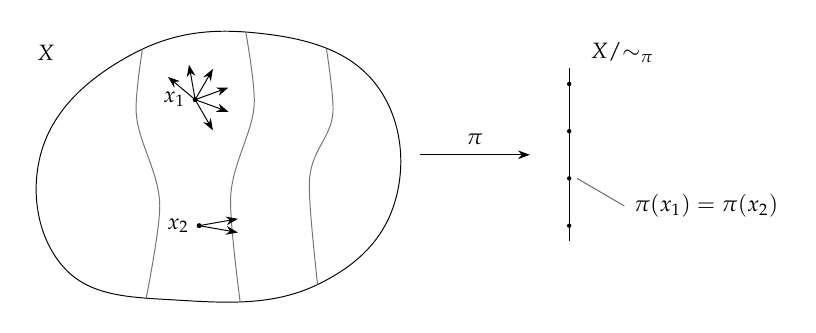
\begin{tikzpicture}[line width=0.35pt, >={Stealth[length=1.5mm,width=1.1mm]}, font=\footnotesize]
\def\region{plot[smooth cycle, tension=0.7] coordinates {(0,0) (1.5,-0.4) (3.2,-0.2) (4.2,0.9) (3.9,2.4) (2.4,3.0) (0.8,2.7) (-0.3,1.5)}}
\draw \region;
\begin{scope}
  \clip \region;
  \draw[black!55] plot[smooth] coordinates {(0.9,-1) (1.2,0.8) (0.9,2.0) (1.1,3.5)};
  \draw[black!55] plot[smooth] coordinates {(2.3,-1) (2.1,0.9) (2.4,2.1) (2.2,3.5)};
  \draw[black!55] plot[smooth] coordinates {(3.3,-1) (3.1,1.1) (3.4,2.0) (3.2,3.5)};
\end{scope}
\coordinate (x1) at (1.65,2.15);
\coordinate (x2) at (1.7,0.55);
\foreach \a in {-60,-20,20,60,100,140}{\draw[->] (x1) -- ++(\a:0.45);}
\foreach \a in {-10,10}{\draw[->] (x2) -- ++(\a:0.5);}
\fill (x1) circle (0.9pt); \fill (x2) circle (0.9pt);
\node[anchor=east, inner sep=2pt] at ($(x1)+(-0.05,0)$) {$x_1$};
\node[anchor=east, inner sep=2pt] at ($(x2)+(-0.05,0)$) {$x_2$};
\node at (-0.25,2.75) {$X$};
\draw[->] (4.5,1.45) -- node[above] {$\pi$} (5.9,1.45);
\draw (6.4,0.35) -- (6.4,2.55);
\foreach \yy in {0.55,1.15,1.75,2.35}{\fill (6.4,\yy) circle (0.8pt);}
\draw[black!60] (6.5,1.15) -- (7.1,0.8) node[anchor=west, black] {$\pi(x_1)=\pi(x_2)$};
\node[anchor=west] at (6.55,2.75) {$X/{\sim_\pi}$};
\end{tikzpicture}
\caption{Quotient geometry. The partition of $X$ is the one induced by $\pi$, and each class collapses to a single point of $X/{\sim_\pi}$. The states $x_1$ and $x_2$ fall in the same class, so $\pi(x_1)=\pi(x_2)$, while their continuation structures differ, $Q(\mathcal{C}(x_1)) \neq Q(\mathcal{C}(x_2))$ for a property $Q$ such as the size of the continuation fan. The compression is then not $Q$-preserving. Schematic.}
\label{fig:quotient}
\end{figure}

\section{Three Missing Terms}

The three cases can now be placed side by side. They do not share a mechanism. A shared mathematical description across domains establishes structural invariance under stated conditions, not metaphysical identity, in the way a diffusion equation appears in heat, populations, and opinions without making them one thing \cite{flyxion-clipboard}. What the cases share is a pattern of inference that fails in each, and each failure isolates a different term.
\begin{align}
\text{Ising machine:}&\quad x \text{ does not determine its transitions,}\\
\text{TVA estimation:}&\quad z \text{ does not determine its measurement,}\\
\text{LLM dialogue:}&\quad \mathcal{L} \text{ does not determine its cause.}
\end{align}

A system description adequate to all three needs more than a state space and an objective. A minimal candidate is the tuple
\begin{equation}
\mathfrak{S} = (X, K, \Gamma, M, \mathcal{L}),
\end{equation}
where $X$ is the state space, $K$ the transition kernel, $\Gamma$ the continuation relation derived from $K$ at a chosen resolution, $M$ the measurement operator, and $\mathcal{L}$ the attractor structure. Energy functions and admissibility conditions, which dominated the discussion of the Ising machine, appear here as particular mechanisms for generating $K$ and hence $\Gamma$. They need not belong to every system; a transition structure does.

The three cases then correspond to three places where a single observable can be produced:
\begin{align}
&W_v \longrightarrow P_{\mathrm{sw}} \longrightarrow P_{\mathrm{flip}} \longrightarrow K && \text{(the kernel is shaped physically)},\\
&c(s) \longrightarrow F_\tau\big[c|_{S_\tau}\big] \longrightarrow \hat{C}_\tau && \text{(the reading is shaped by the task)},\\
&x_t \xrightarrow{\;K_{\mathrm{int}} + K_{\mathrm{bias}}\;} x_{t+1} \longrightarrow \mathcal{L} && \text{(the destination is shaped by the prior)}.
\end{align}
What is called behavior in each case is the composition
\begin{equation}
\boxed{\, y_t = M\big(K^t(x_0)\big) \,}
\end{equation}
where $K^t$ denotes $t$ applications of the kernel to an initial state or distribution. An observer holds $y_t$. The endpoint fallacy is the attempt to read off $x_t$, $K$, or $\mathcal{L}$ from $y_t$ alone. Each of the three papers shows, in its own domain, a case where that reading fails, and each points to what would repair it: a controllable kernel, which the Ising work supplies; a demonstrated invariance of the measurement operator, which the TVA work shows to be still outstanding; and an intervention that moves one target while holding the others fixed, which the dialogue work supplies.

With history made explicit, the full diagram is the following, drawn as a single geometric object in Figure~\ref{fig:composition}:
\begin{equation}
H_t \;\longrightarrow\; x_t \;\xrightarrow[\;\mathcal{C}_t\;]{K_t}\; x_{t+1} \;\xrightarrow{\;M_t\;}\; y_{t+1},
\end{equation}
where $H_t$ is the path by which the system reached $x_t$, and the inferential problem is summarized by
\begin{equation}
y_t \;\not\Rightarrow\; x_t \;\not\Rightarrow\; H_t, \qquad x_t \;\not\Rightarrow\; \mathcal{C}_t(x_t) \ \text{ independently of } K_t .
\end{equation}
Different observational regimes give access to different parts of this diagram. Passive observation yields a trajectory. Repeated initialization from the same state yields an estimate of $K$. Intervention and perturbation are needed for $\Gamma$, $\mathrm{Rev}$, and $\mathcal{L}$, which are inferred from how the system responds to being moved rather than read off its coordinate, in the same way that an admissible region is reconstructed from recovery behavior rather than observed directly \cite{flyxion-clipboard}. The three papers occupy these regimes almost exactly. The Ising work estimates $K$ by repeated initialization, a thousand identical pulses per setting, and then controls it. The TVA work holds the participant fixed and intervenes on $M$. The dialogue work initializes every pair of stances twenty-five times and intervenes on framing and on model weights to locate $\mathcal{L}$ and decompose its causes.

\begin{figure}[t]
\centering
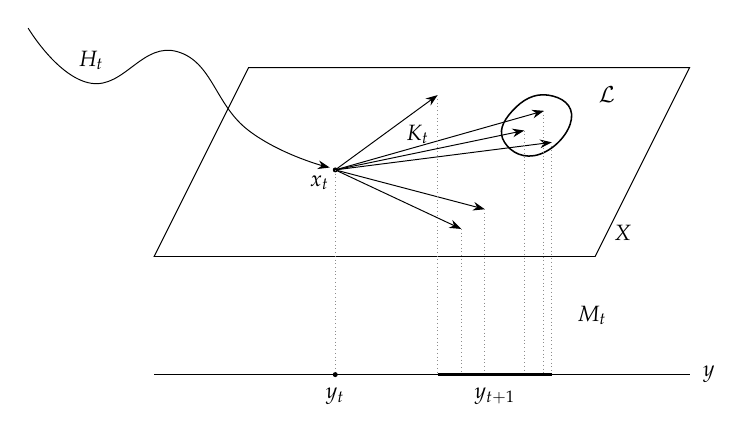
\begin{tikzpicture}[line width=0.35pt, >={Stealth[length=1.5mm,width=1.1mm]}, font=\footnotesize]
\draw (0,0) -- (5.6,0) -- (6.8,2.4) -- (1.2,2.4) -- cycle;
\node at (5.95,0.3) {$X$};
\coordinate (x) at (2.3,1.1);
\draw[->] plot[smooth, tension=0.8] coordinates {(-1.6,2.9) (-0.8,2.2) (0.3,2.6) (1.2,1.6) (2.23,1.13)};
\node[anchor=south] at (-0.8,2.25) {$H_t$};
\draw[line width=0.55pt] plot[smooth cycle, tension=0.85] coordinates {(4.9,1.3) (5.3,1.75) (5.0,2.05) (4.55,1.85) (4.45,1.45)};
\node at (5.75,2.05) {$\mathcal{L}$};
\foreach \e in {(4.7,1.6),(4.95,1.85),(5.05,1.45),(4.2,0.6),(3.6,2.05),(3.9,0.35)}{
  \draw[->] (x) -- \e;
}
\fill (x) circle (0.9pt);
\node[anchor=north east, inner sep=2pt] at (x) {$x_t$};
\node at (3.35,1.55) {$K_t$};
\draw (0,-1.5) -- (6.8,-1.5);
\node[anchor=west] at (6.85,-1.5) {$y$};
\foreach \ex/\ey in {4.7/1.6,4.95/1.85,5.05/1.45,4.2/0.6,3.6/2.05,3.9/0.35}{
  \draw[black!45, densely dotted] (\ex,\ey) -- (\ex,-1.5);
}
\draw[black!45, densely dotted] (x) -- (2.3,-1.5);
\draw[line width=1.1pt] (3.6,-1.5) -- (5.05,-1.5);
\fill (2.3,-1.5) circle (0.9pt);
\node[anchor=north] at (2.3,-1.55) {$y_t$};
\node[anchor=north] at (4.33,-1.55) {$y_{t+1}$};
\node[anchor=west] at (5.25,-0.75) {$M_t$};
\end{tikzpicture}
\caption{The composition $y_t = M(K^t(x_0))$ drawn as one object. A history $H_t$ brings the system to $x_t$ in the state space $X$; the kernel $K_t$ opens a fan of continuations, some of which enter the attractor region $\mathcal{L}$; the measurement $M_t$ projects states onto an observation axis, where the whole fan collapses to an interval. An observer holding points of the axis cannot recover the fan, the history, or which continuations ended in $\mathcal{L}$. Schematic.}
\label{fig:composition}
\end{figure}

Each of the three cases is also an instance of a more general compression. An outcome that depends on an object together with the conditions arranged around it,
\begin{equation}
O = f(x, \Theta),
\end{equation}
is reported as though it depended on the object alone, $O = f(x)$. The annealing schedule and penalty weights are arranged conditions for the Ising machine. The paradigm, stimulus layout, and report instructions are arranged conditions for the TVA estimate. Initialization prompts, statement framing, model weights, and turn order are arranged conditions for the dialogue. Changing the arrangement changes what the trajectory licenses anyone to infer.

A fourth structure runs underneath all three and is easy to miss. Every judgment in the account is made at a resolution. A move is reachable at threshold $\varepsilon$; a kernel can express only as many probability levels as its random source allows, which is consistent with a 4-bit shift register searching worse than a 16-bit one; two estimates are equivalent at tolerance $\delta$; an attractor is located where the drift falls below some magnitude. Some of these resolutions belong to the system, as with the probability levels its random source can express. Others, such as $\varepsilon$, $\delta$, and the drift magnitude at which an attractor is located, are declared by whoever describes it, and different declarations yield different verdicts about the same data.

Collected, the distinctions the essay has argued for, each supported by at least one of the three cases, are these:
\begin{equation}
\begin{aligned}
\text{existence} &\neq \text{reachability},\\
\text{observation} &\neq \text{state},\\
\text{agreement} &\neq \text{interaction},\\
\text{same coordinate} &\neq \text{same continuation},\\
\text{same endpoint} &\neq \text{same history},\\
\text{same parameter name} &\neq \text{same measured quantity}.
\end{aligned}
\end{equation}

The central claim of the essay can be put in one sentence. A state is intelligible only relative to the dynamics that reach it, the measurement that reveals it, and the continuations that remain from it.

\section{Neighboring Frameworks}

Each piece of the argument has a well-developed neighbor, and a reader will recognize them. Energy-landscape theory studies the organization of minima, saddles, and basins \cite{wales2003}; the argument here depends on it and adds only that a landscape underdetermines its kernel. Glauber dynamics and simulated annealing are standard \cite{glauber1963,kirkpatrick1983}, as is the compilation of combinatorial problems into Ising penalties \cite{lucas2014}. The hardware literature increasingly treats problem mapping, schedule, update rule, and device as a co-designed system rather than assuming that the Hamiltonian determines solver behavior \cite{mohseni2022}, and the VSIM paper is an instance of that stance. Dynamical systems theory studies attractors and basins; control theory and viability theory study reachable and viable sets \cite{aubin1991}. Measurement-invariance methodology asks when a construct is measured equivalently across groups or instruments \cite{meredith1993}. Bisimulation and lumpability characterize when states may be merged without loss \cite{kemeny1960,larsen1991,givan2003}. Classical opinion dynamics, from DeGroot averaging through the Friedkin-Johnsen model with its attachment to initial opinions to bounded confidence, supplies the kind of interaction term the dialogue study fits \cite{degroot1974,friedkin1990,hegselmann2002}. The Friedkin-Johnsen model in particular already separates social averaging from a pull toward a fixed prior, and can be read as a linear ancestor of the topic-bias term.

Ecological psychology's affordances \cite{gibson1979} are the closest relative of the continuation set and should be distinguished from it. An affordance is a possibility for action relative to an organism, typically available to its perception. $\Gamma(x)$ need not be perceived by anything; it can describe physically, computationally, or institutionally reachable continuations whether or not any agent sees them. In systems where both can be defined, what is afforded is a subset of what is reachable, and the gap between them is itself informative.

What the essay adds is not a new object in any one of these fields but an account of the inferential relations among them. It asks when $\pi(x)$, $x$, $K$, $\Gamma$, $\mathcal{L}$, and a system's history may stand in for one another, and when they may not. The general answer is that state descriptions are lossy quotients of dynamical systems, and different quotients preserve different claims. Earlier essays in this series approached the same structure from other directions: signals that keep their surface form while losing the maintained inverse mapping that gave them evidential force \cite{flyxion-decoupling}; outcomes attributed to systems whose conditions people supplied, with risk recast as a property of reachable and admitted continuations \cite{flyxion-arranged}; interfaces that expose only some of the technically feasible actions and so bundle changes a user would make separately \cite{flyxion-adjacency}; null ablations read as motion within a fibre of the observation map \cite{flyxion-ablation}; and the separation of a claim's readiness for judgment from an action's permissibility, which turns on the action's reversibility \cite{flyxion-reversibility}.

The closest companion is a monograph on clipboards as re-enterable compressed traversals \cite{flyxion-clipboard}, from which this essay borrows graded transition admissibility, the quotient reading of compression, the entropy taxonomy, and the treatment of admissible regions as inferred rather than observed. The two projects divide the ground. That work asks how traversals survive compression; this one asks what must be known to characterize a traversal at all. The concept between them is continuation-preserving compression, and it gives a precise sense to that work's closing claim that the clipboard is not how we remember but how we continue: to continue is to reconstruct a family of trajectories from whatever part of $\mathcal{C}$ the compression kept.

\section{The Shape of Search}

The word ``search'' is used here in a broadened sense. An Ising machine searches over spin configurations. Attention, in the TVA picture, is a competitive selection among categorizations racing for limited storage. A dialogue between agents traverses a space of stances. The claim is not that these are one process. It is that each is misdescribed by its endpoints in the same way, and that the correction in each case is to recover the structure that endpoints discard.

The opening equation,
\begin{equation}
x^\star = \arg\min_{x \in X} E(x),
\end{equation}
names a destination and erases the journey. Against it stand three relations that no endpoint records:
\begin{equation}
x_t \xrightarrow{\;K\;} x_{t+1}, \qquad x_t \xrightarrow{\;M\;} y_t, \qquad x_t \xrightarrow{\;\Gamma\;} \{x_{t+1}\},
\end{equation}
so that
\begin{equation}
x_t \ \text{ does not identify } \ (K, M, \Gamma).
\end{equation}

The same structure appears well outside laboratories. A machine can physically exist while the repair paths that would keep it in service have been withdrawn by a part no longer sold or a lock that cannot be opened; an option can remain listed while every route to it has been gated; an interface can expose fewer actions than are technically feasible, so that a change a user wants exists and cannot be made on its own \cite{flyxion-adjacency}. In each case the object is in $X$ and absent from $\Gamma(x)$. Existence is not reachability. Search, whether performed by an annealer, an attentional system, a conversation, or an institution, does not merely rank destinations. It manufactures adjacency, deciding which parts of the space count as next.

A coordinate says where a system is only after a space has been chosen. It does not say how the system arrived, which forces shaped the route, how the coordinate became observable, or which departures remain open. These are not commentary on the state. They are the structure that makes the state consequential. An optimizer is not defined only by what it prefers; it is defined by what it can become, and by the schedule on which it stops being able to become anything else.

\appendix
\section{Five Minimal Propositions}

\begin{proposition}[Directional nesting of continuation sets]\label{prop:nest}
Let $K_T$ be a single-spin Glauber kernel with site selection probability $q_i > 0$, so that for the configuration $x^{(i)}$ obtained by flipping spin $i$,
\[
K_T(x^{(i)} \mid x) = q_i \,\big(1 + e^{-\delta H_i(x)/T}\big)^{-1},
\]
where $\delta H_i$ is the energy reduction produced by the flip. For fixed $\varepsilon > 0$ define $\Gamma_T^{\varepsilon,-}(x) = \{ x^{(i)} : \delta H_i(x) < 0,\ K_T(x^{(i)} \mid x) \geq \varepsilon \}$. If $T > T'$ then $\Gamma_{T'}^{\varepsilon,-}(x) \subseteq \Gamma_T^{\varepsilon,-}(x)$.
\end{proposition}
\begin{proof}
For $\delta H_i < 0$ the exponent $-\delta H_i / T = |\delta H_i|/T$ decreases as $T$ increases, so $T \mapsto (1 + e^{|\delta H_i|/T})^{-1}$ is strictly increasing on $(0,\infty)$. Hence $K_{T'}(x^{(i)} \mid x) \geq \varepsilon$ implies $K_T(x^{(i)} \mid x) \geq \varepsilon$.
\end{proof}
\begin{remark}
For $\delta H_i > 0$ the same function is strictly decreasing in $T$, so downhill continuation sets grow as $T$ falls. In the VSIM the realized kernel is further shaped by the pulse-width window: with $W_v = \delta H/(\alpha T) + W_0$ restricted to $[0.3, 1]$\,ns, the achievable flip probabilities are those of the fitted sigmoid over that interval, and required widths outside it are clipped. The effective continuation sets are those of a clipped, device-dependent kernel, not of the ideal Glauber rule.
\end{remark}

\begin{proposition}[Raising one penalty cannot expel the ground state]\label{prop:penalty}
Let $H_\lambda = H_o + \sum_k \lambda_k H_{ck}$ with $H_{ck} \geq 0$ and $H_{ck}(x) = 0$ whenever $C_k(x)$ holds, and let $x^\star \in \A$ be a global minimizer of $H_\lambda$. If $\lambda'$ agrees with $\lambda$ except that $\lambda'_m > \lambda_m$ for one index $m$, then $x^\star$ is a global minimizer of $H_{\lambda'}$.
\end{proposition}
\begin{proof}
$H_{\lambda'}(x) = H_\lambda(x) + (\lambda'_m - \lambda_m) H_{cm}(x) \geq H_\lambda(x) \geq H_\lambda(x^\star) = H_{\lambda'}(x^\star)$, the last equality because $H_{cm}(x^\star) = 0$.
\end{proof}
\begin{remark}
The hypotheses hold for the routing penalties. $H_{c1}$ and $H_{c4}$ are sums of squares and of nonnegative terms. Each summand of the first part of $H_{c2}$ takes values in $\{0,1\}$ on binary variables, and the second part is a sum of nonnegative products. In $H_{c3}$, a Steiner vertex with $k \geq 2$ incoming and $m \leq |V|$ outgoing arcs contributes $|V|\binom{k}{2} - (k-1)m \geq (k-1)(|V| - m) \geq 0$, and all terms vanish on configurations satisfying their constraints in the enlarged space of edge and order variables. Any increase in invalid outcomes observed when a single penalty weight is raised, as for $\lambda_3$ in the routing sensitivity analysis, is therefore, whenever the ground state before the change was admissible, a property of finite-time dynamics under the deformed landscape, not of the location of its minimum.
\end{remark}

\begin{proposition}[Non-injective projection with distinct response]\label{prop:proj}
Let stances take values in $\{-1, 0, 1\}$, and let $p = (0, 1, 0)$ and $r = (\tfrac12, 0, \tfrac12)$ be two distributions over them. Then $\E_p[X] = \E_r[X] = 0$ while $H(p) = 0$ and $H(r) = \log 2$. Moreover, for the mixing update $p \mapsto (1-\alpha)p + \alpha\,\delta_{1}$ with $0 < \alpha < 1$, representing partial movement toward the stance $+1$, both expectations become $\alpha$, but the probability assigned to the opposed stance $-1$ is $0$ in the first case and $(1-\alpha)/2$ in the second.
\end{proposition}
\begin{proof}
Direct computation.
\end{proof}
\begin{remark}
Even a perturbation that moves both expectations identically leaves the two agents in different states with respect to the opposed response. Any dynamics whose next step depends on more than the mean will separate them further, so the scalar projection cannot serve as a state variable for such dynamics. The empirical correlation between response entropy and the variance of the next opinion shift reported by Brockers, Ehrlich, and Priesemann is evidence that language-model dialogue is dynamics of this kind. Adding a second statistic does not close the gap in general: on $\{-2,-1,0,1,2\}$, the distributions $(\tfrac12,0,0,0,\tfrac12)$ and $(0,\tfrac12,0,\tfrac12,0)$ share mean $0$ and entropy $\log 2$, while their variances are $4$ and $1$.
\end{remark}


\begin{proposition}[Endpoint non-identifiability of linear pulls]\label{prop:centroid}
Let a scalar state evolve under drift $\dot{x} = \sum_{k=1}^{n} \beta_k (b_k - x)$ with $\beta_k > 0$. Then $x(t) \to \bar{b} = \sum_k \beta_k b_k / \sum_k \beta_k$ from every initial condition. For any $n \geq 2$ and any $\bar{b}$, there are infinitely many parameter vectors $(\beta, b)$ with the same limit, so the limit determines neither the weights nor the targets.
\end{proposition}
\begin{proof}
The drift equals $B(\bar{b} - x)$ with $B = \sum_k \beta_k > 0$, whose unique globally attracting fixed point is $\bar{b}$. For fixed $\bar{b}$, the constraint $\sum_k \beta_k (b_k - \bar{b}) = 0$ is one equation in $2n$ unknowns.
\end{proof}
\begin{remark}
The trajectory reveals more than the endpoint, since the convergence rate recovers $B$, but even the full trajectory of the one-dimensional system determines only $B$ and $\bar{b}$. Separating individual terms requires interventions that move targets differently. Negating the statement maps $b_{\mathrm{top}} \mapsto -b_{\mathrm{top}}$ while fixing the agreement target at $+2$, so comparing the two framings recovers $\beta_{\mathrm{agr}}$ and $\beta_{\mathrm{top}} b_{\mathrm{top}}$ separately, which is how negated framing separates the two terms. The authors' recovery study includes a synthetic scenario in which the topic attractor coincides with the agreement target, the degenerate case of this proposition within a single framing, and reports recovery across its scenarios. In their response to reviewers the authors give the reason in terms close to the ones used here: the topic term acts on a framing-sensitive target, the agreement term on a target that ignores framing, and the anchoring term only on the responding agent, so the three apply differently to different observations \cite{brockers2026peer}. Negated framing, fixed targets, and asymmetric application are the interventions that break the degeneracy the proposition describes. Time-decaying coefficients, as in the fitted model, add further leverage when their timescales differ.
\end{remark}


\begin{proposition}[Lumpability]\label{prop:lump}
Let $(x_t)$ be a Markov chain on a finite set $X$ with kernel $K$, and let $\pi : X \to Y$. The process $y_t = \pi(x_t)$ is a Markov chain with the same transition matrix for every initial distribution if and only if, for every $y, y' \in Y$, the block probability
\[
K\big(\pi^{-1}(y') \mid x\big) = \sum_{x' \in \pi^{-1}(y')} K(x' \mid x)
\]
takes the same value for all $x \in \pi^{-1}(y)$.
\end{proposition}
\begin{proof}
This is the strong lumpability theorem of Kemeny and Snell \cite{kemeny1960}.
\end{proof}
\begin{remark}
When the condition fails, there are states $x, x'$ with $\pi(x) = \pi(x')$ whose next-observation distributions differ. Conditioning on $y_t$ alone then need not determine the law of $y_{t+1}$ independently of the hidden-state distribution within its block. Particular initial distributions can still yield a Markov projected process (weak lumpability), and $y_t$ remains a legitimate descriptive variable; what fails is a single transition law valid for all of them. The largest observation-compatible bisimulation is the coarsest refinement of the $\pi$-partition that is itself lumpable; when the $\pi$-partition is already lumpable, it is that bisimulation.
\end{remark}

\begin{thebibliography}{9}

\bibitem{li2026}
S.~Li, Y.~Zhang, A.~Lee, Z.~Zhu, L.~Zeng, P.~Wang, L.~Gao, D.~Wu, and W.~Zhao.
An Ising machine for combinatorial optimization based on sub-nanosecond CMOS-integrated magnetoresistive random-access memory.
\emph{Nature Electronics}, 2026.
doi:10.1038/s41928-026-01700-6.

\bibitem{biermeier2026}
K.~Biermeier and I.~Scharlau.
Comparing attention estimates across two tasks through formalization.
\emph{Scientific Reports}, 16:29499, 2026.
doi:10.1038/s41598-026-71598-9.

\bibitem{brockers2026}
V.~C. Brockers, D.~A. Ehrlich, and V.~Priesemann.
Disentangling interaction and bias effects in opinion dynamics of large language models.
\emph{Nature Communications}, 17:10077, 2026.
doi:10.1038/s41467-026-77340-3.

\bibitem{bundesen1990}
C.~Bundesen.
A theory of visual attention.
\emph{Psychological Review}, 97(4):523--547, 1990.


\bibitem{glauber1963}
R.~J. Glauber.
Time-dependent statistics of the Ising model.
\emph{Journal of Mathematical Physics}, 4:294--307, 1963.

\bibitem{kirkpatrick1983}
S.~Kirkpatrick, C.~D. Gelatt, and M.~P. Vecchi.
Optimization by simulated annealing.
\emph{Science}, 220:671--680, 1983.

\bibitem{lucas2014}
A.~Lucas.
Ising formulations of many NP problems.
\emph{Frontiers in Physics}, 2:5, 2014.

\bibitem{mohseni2022}
N.~Mohseni, P.~L. McMahon, and T.~Byrnes.
Ising machines as hardware solvers of combinatorial optimization problems.
\emph{Nature Reviews Physics}, 4:363--379, 2022.

\bibitem{wales2003}
D.~J. Wales.
\emph{Energy Landscapes}.
Cambridge University Press, 2003.

\bibitem{aubin1991}
J.-P. Aubin.
\emph{Viability Theory}.
Birkh\"auser, 1991.

\bibitem{meredith1993}
W.~Meredith.
Measurement invariance, factor analysis and factorial invariance.
\emph{Psychometrika}, 58:525--543, 1993.

\bibitem{kemeny1960}
J.~G. Kemeny and J.~L. Snell.
\emph{Finite Markov Chains}.
Van Nostrand, 1960; 2nd ed., Springer, 1976. Lumpability is treated in Chapter~VI.

\bibitem{larsen1991}
K.~G. Larsen and A.~Skou.
Bisimulation through probabilistic testing.
\emph{Information and Computation}, 94(1):1--28, 1991.
doi:10.1016/0890-5401(91)90030-6.

\bibitem{givan2003}
R.~Givan, T.~Dean, and M.~Greig.
Equivalence notions and model minimization in Markov decision processes.
\emph{Artificial Intelligence}, 147:163--223, 2003.

\bibitem{li2006}
L.~Li, T.~J. Walsh, and M.~L. Littman.
Towards a unified theory of state abstraction for MDPs.
In \emph{Proceedings of the International Symposium on Artificial Intelligence and Mathematics}, 2006.

\bibitem{degroot1974}
M.~H. DeGroot.
Reaching a consensus.
\emph{Journal of the American Statistical Association}, 69:118--121, 1974.

\bibitem{friedkin1990}
N.~E. Friedkin and E.~C. Johnsen.
Social influence and opinions.
\emph{Journal of Mathematical Sociology}, 15:193--206, 1990.

\bibitem{hegselmann2002}
R.~Hegselmann and U.~Krause.
Opinion dynamics and bounded confidence: models, analysis, and simulation.
\emph{Journal of Artificial Societies and Social Simulation}, 5(3), 2002.

\bibitem{gibson1979}
J.~J. Gibson.
\emph{The Ecological Approach to Visual Perception}.
Houghton Mifflin, 1979.

\bibitem{flyxion-decoupling}
Flyxion.
Evidentiary decoupling: signal-outcome alignment in neurodevelopmental regulation and capability assessment.
Essay, September 2026.

\bibitem{flyxion-arranged}
Flyxion.
Arranged conditions: two accounts of the same fear.
Essay, September 2026.

\bibitem{flyxion-adjacency}
Flyxion.
The unchosen adjacency.
Essay, September 2026.

\bibitem{flyxion-ablation}
Flyxion.
Ablation invariance: what null ablations reveal about hidden architecture.
Essay, September 2026.

\bibitem{flyxion-reversibility}
Flyxion.
The reversibility gate: evidence, delay, and action under unsettled claims.
Essay, September 2026.

\bibitem{flyxion-clipboard}
Flyxion.
\emph{Everything Is a Clipboard: Recursive State, Functional Essays, and the Computational Geometry of Externalized Cognition}.
Monograph, 2026.
\url{https://standardgalactic.github.io/alphabet/framework/everything_is_a_clipboard.pdf}.

\bibitem{mackenzie1983}
N.~D. Mackenzie and A.~P. Young.
Statics and dynamics of the infinite-range Ising spin glass model.
\emph{Journal of Physics C: Solid State Physics}, 16:5321--5337, 1983.

\bibitem{brockers2026peer}
V.~C. Brockers, D.~A. Ehrlich, and V.~Priesemann.
Peer review file for ``Disentangling interaction and bias effects in opinion dynamics of large language models''.
\emph{Nature Communications}, 17:10077, 2026, supplementary material.

\bibitem{tunnermann2015}
J.~Tünnermann, A.~Petersen, and I.~Scharlau.
Does attention speed up processing? Decreases and increases of processing rates in visual prior entry.
\emph{Journal of Vision}, 15(3):1, 2015.
doi:10.1167/15.3.1.

\end{thebibliography}

\end{document}
